% This file is part of Bachelorarbeit

% Bachelorarbeit is free software: you can redistribute it and/or modify
% it under the terms of the GNU General Public License version 3 as published by
% the Free Software Foundation.

% Bachelorarbeit is distributed in the hope that it will be useful,
% but WITHOUT ANY WARRANTY; without even the implied warranty of
% MERCHANTABILITY or FITNESS FOR A PARTICULAR PURPOSE.  See the
% GNU General Public License for more details.

% You should have received a copy of the GNU General Public License
% along with Foobar. If not, see <http://www.gnu.org/licenses/>.

\section{Vorgehensweise}

Zuerst wurden alle nötigen Änderungen ausfindig gemacht. Dies beinhaltete
die Migrierung von Code von UNIX/Linux-spezifischem IO-Multiplexing
mittels poll() zu anderen Verfahren.

Des weiteren mussten fehlende Features gefunden werden. Einen Hinweis
darauf ließ sich bereits auf den Wiki-Seiten über die Plugins für Windows finden.
Dieser ergab, dass die Verwaltung von virtuellen IPs unter Windows momentan
nicht unterstützt wurde.

Weitere Punkte wurden nach dem ersten Kompilierungsversuch, sowie der Beobachtung
des Verhaltens während dem Tunnelaufbau herausgefunden.

Die Unterstützung für virtuelle IP-Adressen wurden aus dem Zweig \texttt{win-vip}
vom strongSwan Git-Repository bezogen und angepasst. Der Großteil des Quellcodes
stammt also von Martin Brunner, der diesen Code geschrieben hat. Der Code musste
noch um die Beachtung eines Konfigurationswertes ergänzt werden.

Die Installation der Routen in kernel-libipsec wurde angepasst, sodass es
mit dem TAP-Treiber funktioniert.

\begin{figure}[!ht]
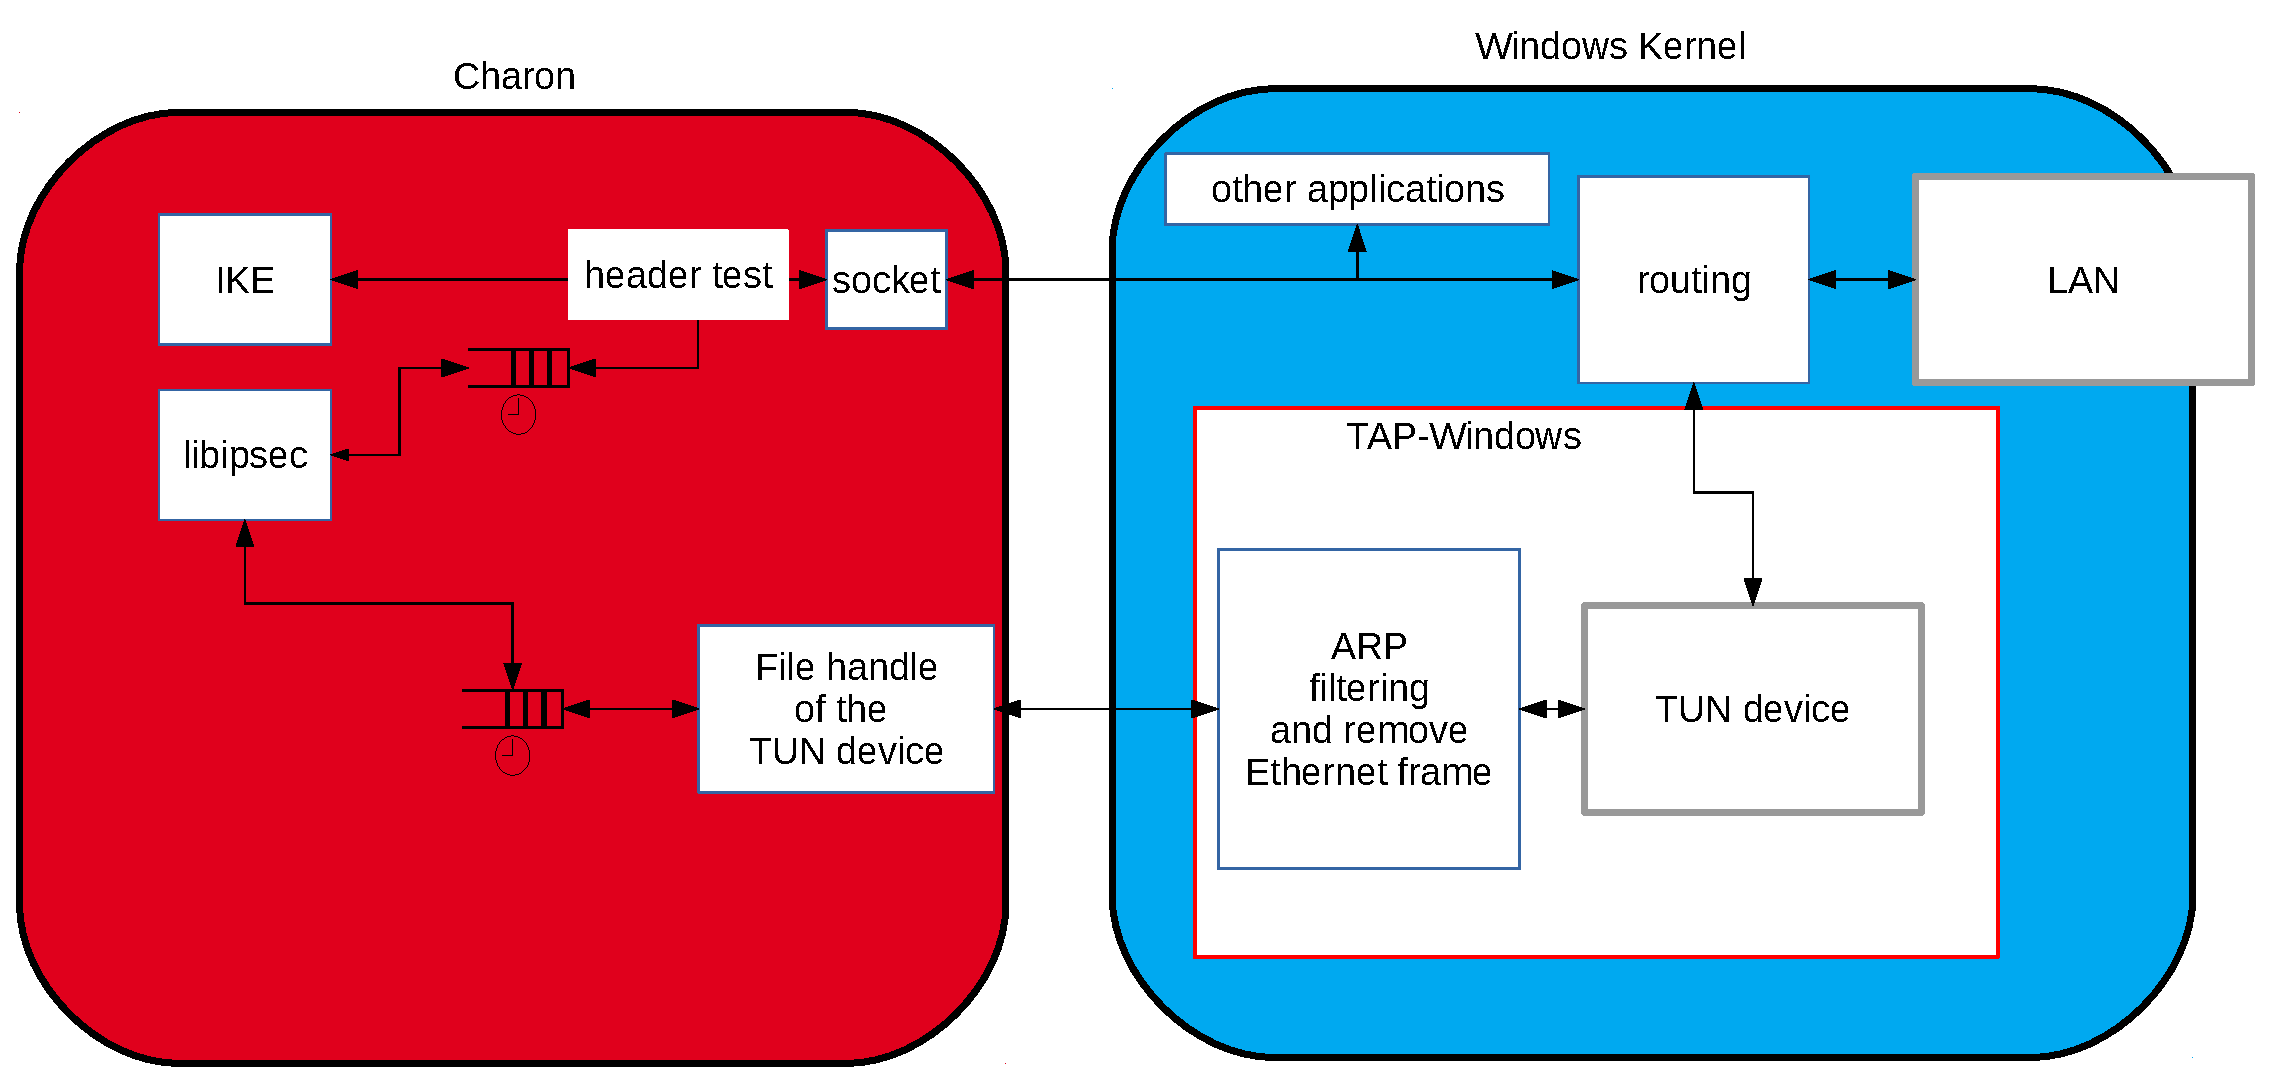
\includegraphics[width=\textwidth]{Diagram.eps}
\caption{Datenflussdiagramm}
\label{fig:Datenflussdiagramm}
\end{figure}

\subsection{Portierung von libipsec auf Windows}
Die Portierung von libipsec auf Windows, sodass sie dort lauffähig ist, ist das Ziel
der Bachelorarbeit. Die zu portierenden Teile des Programmcodes betreffen nur
die Codesegmente, die Plattformspezifische \acp{API} oder \acp{ABI} verwenden,
also primär alles um Dateiein- und Ausgabe, sowie das Verwalten von TUN-Geräten.
Unter Unix und Linux werden hier \acp{FD} verwendet. Unter Windows werden stattdessen
Handles genutzt, welche einen anderen Dateityp darstellen. Des weiteren unterscheidet
sich die Methode zum Multiplexen von Lese-Aufrufen auf einer Liste von Handles oder \acp{FD} stark.
Unter Unix und Linux wird hierfür poll() genutzt, unter Windows geschieht das jedoch
Event-basiert mit WaitForMultipleObjects().
Explizite Beispiele hierfür sind im Abschnitt über die Portierung von libipsec sichtbar.
Bei der Portierung wurde für das Verwalten von Speicherabschnitten 
primär alloca() genutzt, statt malloc() und seine Unterarten. Der Unterschied hierbei ist die
Speicherdauer. Mit alloca() allokierter Speicher ist nur bis zum Verlassen der Funktion gültig
und wird automatisch freigegeben. Mit malloc() allokierter Speicher muss manuell freigegeben werden.
alloca() ist ein Feature, welches nicht standardisiert ist.
Daher lässt sich strongSwan nicht mit allen C-Bibliotheken übersetzen.
Auf der Wiki-Seite über den Windows-Port wird erwähnt, dass nur die Kompilierung
mittels MinGW-W64 unterstützt wird.\footcite[][]{_windows_2015}


\subsection{Bestehende Implementierung}
Die bestehende Implementierung umfasst die eigentliche Bibliothek, eine Implementierung
eines Kernel-Interface zwischen libipsec und \texttt{charon}, sowie Code in libstrongswan
um TUN-Geräte zu öffnen. Martin Willi hat 2014 bereits die gesamte Portierungsarbeit
für version 5.2.0 von strongSwan gemacht. Der Port unterstützt Windows 7 / server 2008 R2
und neuere Versionen von Microsoft Windows.

\subsection{Unterstützte Kryptographie}
Die unterstützte Kryptographie ist notwendigerweise von den deklarierten Identifikatoren
für IKE beschränkt. strongSwan unterstützt mehr Verschlüsselungsalgorithmen als
in den \acp{RFC} deklariert wurde. Aus diesem Grund nutzt strongSwan Identifikatoren
teilweise aus dem privaten Bereich, wenn die Identifikatoren für den eingesetzten Algorithmus
nicht standardisiert sind.

strongSwan unterstützt eine große Anzahl von Algorithmen im Vergleich zu anderen Implementierungen,
wie in den Tabellen in \autoref{sec:appendix} dagelegt wird. Wenn libipsec genutzt wird,
so können alle Algorithmen, die im Userspace implementiert sind, für die Absicherung
von Verkehr genutzt werden.

\subsection{Portierung}
\subsubsection{libipsec}
libipsec implementiert die Verarbeitung von Paketen, das Erzwingen der \acp{SP},
das Verwalten der \acp{SP}, \acp{SA}, Routen und der TUN-Geräte.
Die hierbei relevanten Dateien sind unter ''/src/libipsec/'' zu finden.

Standardmäßig installiert strongSwan die IP-Adressen die per Config-Mode
oder \ac{CP} empfangen wird auf dem ausgehenden Interface (Linux, Kernelspace processing),
was für die Kommunikation mit dem Peer genutzt wird,
oder auf dem Loopback-Adapter (Windows).
Um die IP-Adresse für TUN-Geräte korrekt zu setzen, nutzt libipsec den Parameter
\texttt{charon.install\_virtual\_ip\_on} von strongswan.conf, der während der Initialisierung
des Plugins gesetzt wird.
% route installation
% queues
% processing
% event driven
% job
\paragraph{Header}
Die Bibliotheken und Plugins um libipsec nutzen diverse Datenstrukturen und Konstanten,
die in C-Header-Dateien von Linux definiert sind. Diese sind unter Windows nicht verfügbar.
Aus diesem Grund wurde eine Kopie der relevanten Definitionen in den Quellcode kopiert
und fehlende Teile ergänz.
Spezifisch wurde aus dem Quellcode von GLIBC die Definition eines \ac{IP}v4-Headers
und eines \ac{IP}v6-Headers kopiert und die fehlenden Protokollkonstanten per Hand ergänzt.

Ursprünglich wurden diese in ''src/libipsec/win32.h'' abgelegt und in ''src/libpsec/ip\_packet.h'' und ''src/libipsec/ip\_packet.c''
inkludiert. Dabei wurden die Header aus den Headern des Kernels oder den Headenr der GNU LIBC kopiert.
Als Name für das Ifdef-Guard wurde \texttt{WINDOWS\_32\_PROTOCOL\_HEADERS} gewählt. Ein Ifdef-Guard wird benötigt um das Reimportieren
von Header-Dateien in C zu unterbinden. Wenn eine Header-Datei erneut importiert wird,
dann führt das dazu, dass die Kompilierung abbricht, da eine Variable redefiniert wird.
Die Redefinierung einer Variable produziert in C eine Warnung oder einen Fehler.
C-Code wird in der Regel mit dem Argument ''-Wall'' kompiliert, welches
alle Warnungen zu Fehlern umwandelt. Das wird getan, um Warnungen nicht zu übersehen.
Der Compiler generiert Warnungen, wenn er Programmierfehler erkennt,
die berichtenswert sind, aber kein größeres Hinderniss für die Kompilierung sind.

Die Header wurden am Ende der \ac{BA} verändert, sodass sie nicht mehr unter der GPL stehen,
sondern unter der MIT-Lizenz. Das wurde getan, um die Änderungen ins Projekt eintragen zu können.

\begin{lstlisting}[caption=win32.h-Headerdatei für den TAP-Windows6-Treiber,label=win32.h]
#ifndef WIN32_H
#define WIN32_H

#define TAP_WIN_COMPONENT_ID "tap0901"

#define ADAPTER_KEY "SYSTEM\\CurrentControlSet\\Control\\Class\\{4D36E972-E325-11CE-BFC1-08002BE10318}"

/*
 * ======================
 * Filesystem prefixes
 * ======================
 */

#define USERMODEDEVICEDIR "\\\\.\\Global\\"
#define TAP_WIN_SUFFIX    ".tap"

/*
 * TAP IOCTL constants and macros.
 *
 */
#define TAP_WIN_CONTROL_CODE(request,method) \
  CTL_CODE (FILE_DEVICE_UNKNOWN, request, method, FILE_ANY_ACCESS)

/* Present in 8.1 */

#define TAP_WIN_IOCTL_GET_MAC               TAP_WIN_CONTROL_CODE (1, METHOD_BUFFERED)
#define TAP_WIN_IOCTL_GET_VERSION           TAP_WIN_CONTROL_CODE (2, METHOD_BUFFERED)
#define TAP_WIN_IOCTL_GET_MTU               TAP_WIN_CONTROL_CODE (3, METHOD_BUFFERED)
#define TAP_WIN_IOCTL_GET_INFO              TAP_WIN_CONTROL_CODE (4, METHOD_BUFFERED)
#define TAP_WIN_IOCTL_CONFIG_POINT_TO_POINT TAP_WIN_CONTROL_CODE (5, METHOD_BUFFERED)
#define TAP_WIN_IOCTL_SET_MEDIA_STATUS      TAP_WIN_CONTROL_CODE (6, METHOD_BUFFERED)
#define TAP_WIN_IOCTL_CONFIG_DHCP_MASQ      TAP_WIN_CONTROL_CODE (7, METHOD_BUFFERED)
#define TAP_WIN_IOCTL_GET_LOG_LINE          TAP_WIN_CONTROL_CODE (8, METHOD_BUFFERED)
#define TAP_WIN_IOCTL_CONFIG_DHCP_SET_OPT   TAP_WIN_CONTROL_CODE (9, METHOD_BUFFERED)

/* Added in 8.2 */

/* obsoletes TAP_WIN_IOCTL_CONFIG_POINT_TO_POINT */
#define TAP_WIN_IOCTL_CONFIG_TUN            TAP_WIN_CONTROL_CODE (10, METHOD_BUFFERED)
#define TAP_WIN_IOCTL_CONFIG_SET_SRC_CHECK  TAP_WIN_CONTROL_CODE (11, METHOD_BUFFERED)


#endif /* WIN32_H */
\end{lstlisting}
Die Headerdatei ''win32.h'' definiert verschiedene Makros für die Kommunikation mit und Konfiguration
des TAP-Windows6-Treibers.

Das Makro \texttt{TAP\_WIN\_COMPONENT\_ID} mit Wert 'tap0901'' wird genutzt, um in der Registry
valide TAP-Geräte unter den Netzwerkverbindungen zu finden. Dabei wird der String-Wert \texttt{ComponentId}
überprüft. Wenn sein Inhalt ''tap0901'' ist, dann ist das Gerät ein valides TAP-Gerät.

Die existierenden Netzwerkadapter können unter {HKEY\_LOCAL\_MACHINE\linebreak
\textbackslash{}SYSTEM\textbackslash{}CurrentControlSet\textbackslash{}Control
\textbackslash{}Class\textbackslash{}\{4D36E972-E325-11CE-BFC1-08002BE10318\} gefunden werden.

\begin{figure}[!h]
\caption{Registry-Eintrag über ein TAP-Gerät}
\label{fig:registry-tap-device}
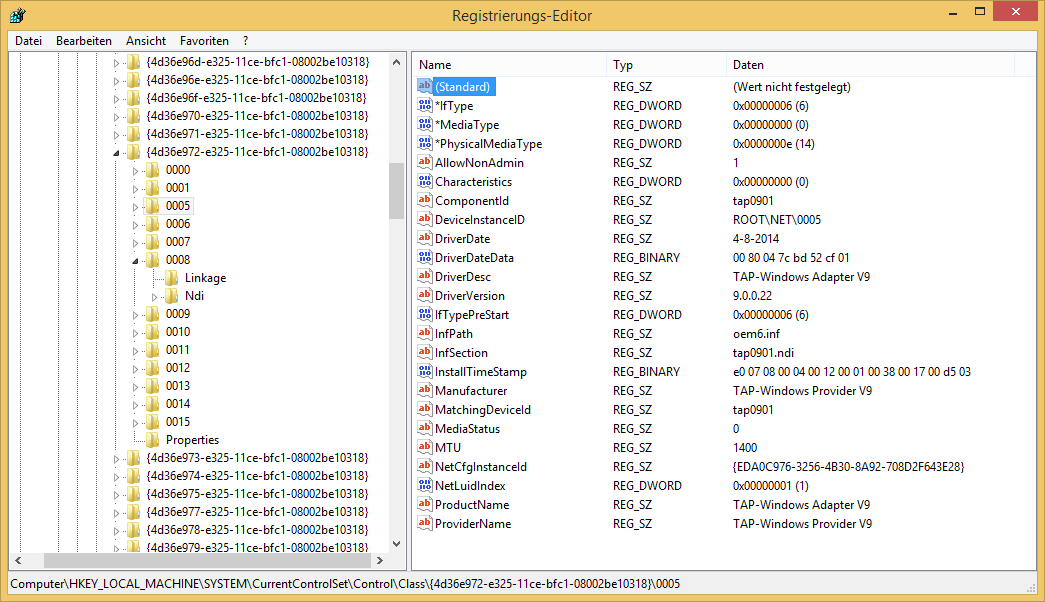
\includegraphics[width=\textwidth]{Windows-Registry-TAP-Device.png}
\end{figure}

In~\autoref{fig:registry-tap-device} sind die verschiedenen Einträge eines Geräts unter
dem oben genannten Pfad zu sehen beispielhaft an einem TAP-Gerät zu sehen. Das TAP-Gerät
wurde mit dem TAP-Windows6-Treiber erstellt.

\begin{figure}[!h]
\caption{Netzwerkverwaltung eines TAP-Geräts}
\label{fig:networkmanager-extended}
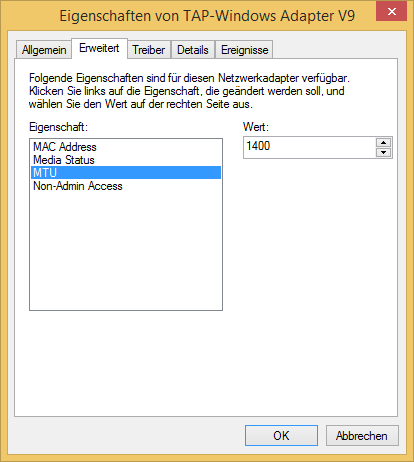
\includegraphics{Windows-NetworkManager-Extended.png}
\end{figure}

In~\autoref{fig:networkmanager-extended} sind die vom Benutzer konfigurierbaren Optionen zu sehen.
Sie werden als Werte in der Registry gespeichert und können auch dort verändert werden.

Die Makros USERMODEDEVICEDIR und TAP\_WIN\_SUFFIX werden zusammen mit der GUID des Geräts
genutzt, um ein Handle im Geräteverzeichnis zu erstellen. Der sich daraus ergebende Pfad
wird genutzt, um ein Handle zu erstellen, welches der TAP-Windows6-Treiber nutzt, um
mit dem Programm im Userspace zu kommunizieren und umgekehrt.

Die Definitionen, die mit TAP\_WIN\_IOCTL beginnen definieren die Werte, die mit
IoCtl benutzt werden können, um das TAP-Gerät zu konfigurieren. Details über die verschiedenen
Werte sind in~\autoref{fig:tap-ioctls} zu finden.


\subsubsection{kernel-libipsec}
Die primäre Aufgabe hier war die Installation der Routen in \texttt{kernel\_libipsec\_ipsec.c}
für Windows anzupassen, da hier ein Gateway verwendet wird auf einem TAP-Gerät
statt ein echtes TUN-Gerät, sowie die Anpassung des Codes für die Ein- und Ausgabe 
und einige Methoden in
\texttt{kernel\_libipsec\_router.c} da das Multiplexen der Handles, sowie die Benachrichtigung
von anderen Threads auf Windows anders abläuft als auf Linux und UNIX.

\paragraph{Multiplexing}
Für das Multiplexen der Eingabe stehen unter Windows zwei Verfahren zur Verfügung:
\begin{itemize}
\item WaitForMultipleObjects
\item IOCompletionPorts
\end{itemize}

WaitForMultipleObjects\footcite[][]{_waitformultipleobjects_2016} funktioniert mit einem Array aus Handles. In der Struktur des Handles
ist das event-Attribut auf ein einzgartiges Event gesetzt, welches genutzt wird um
das Handle zu finden, dessen Lesevorgang abgeschlossen oder abgebrochen wurde.
Nach dem Kopieren des Handles in das Array und dem Setzen des Events wird ein asynchroner
Lesevorgang gestartet. Wenn er sofort beendet wurde, wird das entsprechende Event gesetzt.
Dadurch beendet der Aufruf von WaitForMultipleObjects() nach dem Aufruf direkt, falls
ein Lesevorgang schon zuvor erfolgreich war und der Programmcode wird etwas kürzer.
% Mehr Erläuterung benötigt

IOCompletionPorts\footcite[][]{_createiocompletionport_2016} funktionieren, indem man einen IOCompletionPort mit CreateIoCompletionPort()
anlegt und Handles mit ihm asoziiert. Bei der Asoziierung wird ein einzigartiger Schlüssel
übergeben, der bei der Signalisierung wieder zurückgegeben wird um das Handle identifizieren zu können.
Der CompletionPort kann erst nach dem Schließen der asoziierten Handles geschlossen werden.
Mit der Funktion GetQueuedCompletionStatus() kann der ausführende Thread dann auf abgeschlossene
I/O-Operationen warten.
Die Nachteile dieser Methode sind, dass jegliche Operationen auf den Handles eine Benachrichtigung
an GetQueuedCompletionStatus() generieren, obwohl Schreib-Vorgänge nicht von Interesse sind.

Des weiteren ähnelt die Nutzung von WaitForMultipleObjects() deren von poll()
insoweit, dass die Handles/\acp{FD} auch nach der Benutzung mit der Funktion
weiterhin einzeln genutzt werden können.
% Mehr Erläuterung benötigt

Da es relativ einfach ist WaitForMultipleObjects() zu nutzen, wurde diese Methode
für die Implementierung von handle\_plain() genutzt.

Die Zustände der Originalimplementierung sind in ~\autoref{fig:poll_fd}
dargestellt.

\begin{figure}
\centering
\def\svgwidth{\columnwidth}
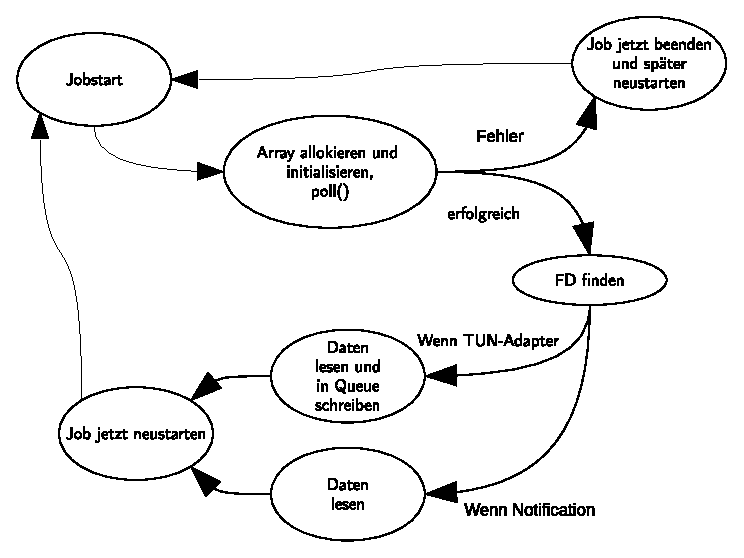
\includegraphics[width=\textwidth]{poll_fd.eps}
\caption{Zustände in handle\_plain() mittels poll()}
\label{fig:poll_fd}
\end{figure}


Wie aus dem Diagramm hervorgeht, wird im Prinzip nur ein Array mit Strukturen des Typs
\texttt{pollfd} erstellt, dann mit einem Notification-\ac{FD} und den \acp{FD} der TUN-Geräte befüllt
und als gewünschte Events \texttt{POLLIN} gesetzt. Das heißt, dass der Aufruf von poll() ohne
Fehler beendet wird, wenn Daten auf dem \acp{FD} zur Verfügung stehen.
Danach wird poll() auf die \texttt{pollfd}-Datenstruktur ausgeführt und analysiert,
auf welchen \acp{FD} Daten zur Verfügung stehen. Dieser Code ist relativ kurz im
Vergleich zum Analogon mit WaitFor*Objects() Funktionen unter Windows.
Dies geht aus den vergleichbaren Implementierungsmöglichkeiten, die sich aus den
WaitFor*Objects()-Funktionen ergeben. Dies wird im Diagramm \autoref{fig:WaitForMultipleObjects}
und \autoref{fig:WaitForMultipleObjects2} hervor. Diese Diagramme haben weitaus
mehr Zustände als \autoref{fig:poll_fd}.

Der Unterschied zwischen der Implementierung von \autoref{fig:WaitForMultipleObjects}
und \autoref{fig:WaitForMultipleObjects2} ist, dass \autoref{fig:WaitForMultipleObjects2}
effektiver und schneller ist, da die Puffer nach jedem Lesevorgang beibehalten werden
und IO-Operationen weiterlaufen können.
In \autoref{fig:WaitForMultipleObjects} werden die Puffer und Operationen
immer freigegeben und gestoppt. Das ist unnötig, bringt die Implementierung
jedoch näher an das Verhalten von \autoref{fig:poll_fd}.
Es wurde das Verfahren aus \autoref{fig:WaitForMultipleObjects2} implementiert,
da es schneller und effektiver ist.

In handle\_plain werden zwei verschiedene Arrays benutzt.
\begin{description}
\item[bundle\_array] Ein Array aus Strukturen vom Typ \texttt{handle\_overlapped\_buffer\_t}. 
\item[event\_array] Ein Array aus Events (HANDLE).
\end{description}

Strukturen vom Typ \texttt{handle\_overlapped\_buffer\_t} beinhalten jeweils ein Objekt
vom Typ HANDLE, ein Objekt vom Typ *OVERLAPPED und ein Objekt vom Typ chunk\_t.
Das Handle gehört zu einem TUN-Handle, das OVERLAPPED-Objekt wird direkt für asynchrones
IO benötigt und das Objekt vom Typ chunk\_t beinhaltet den Pufferspeicher und dessen Länge.

Das \texttt{event\_array} Array zum Multiplexen mittels WaitForMultiplEvents() genutzt und
beinhaltet die gleichen Events, wie die Strukturen des Typs OVERLAPPED.
Bei der Ausführung von WaitForMultipleObjects() auf das Array wird darauf gewartet, dass
eine vorher gestartete Leseoperation auf einem Handle fertig gestellt wird.
Das signalisiert ein Event im Array und dessen Position im Array verrät welche
Position im bundle\_array einen nun gefüllten Puffer hat. Die Position signalisiert
hierbei nur die niedrigste Position im Array, deren Event signalisiert wurde. Ein
im Array höher gelegenes Event könnte auch signalisiert sein.
Der Puffer kann nun gelesen
werden und an die Queue zu libipsec gehängt werden. Nach dem Lesen wird die OVERLAPPED-Struktur
und das Event zurückgesetzt, sowie der Puffer mit Nullen initialisiert und die Länge zurückgesetzt.
Danach wird ein neuer Lesevorgang auf dem oder den Handles gestartet, deren Leseoperationen
fertig sind.

Der Code auf Seite \pageref{lst:handle-plain-windows} zeigt die Implementierung von handle\_plain()
auf Windows. Die Funktionen zum Starten von asynchronen Leseoperationen auf Handles
wurden in start\_read() abgekapselt. Das Übersetzen von Fehlercodes in menschenlesbare
Texte wurde in format\_error() abgekapselt. Bei Fehlern beim Lesen startet sich der Job
mit JOB\_REQUEUE\_FAIR neu, sodass der Job als letzter vom Job-Manager in \texttt{charon} neugestartet wird,
wenn hoffentlich der Fehler nicht erneut auftritt.

\begin{figure}
\centering
\def\svgwidth{\columnwidth}
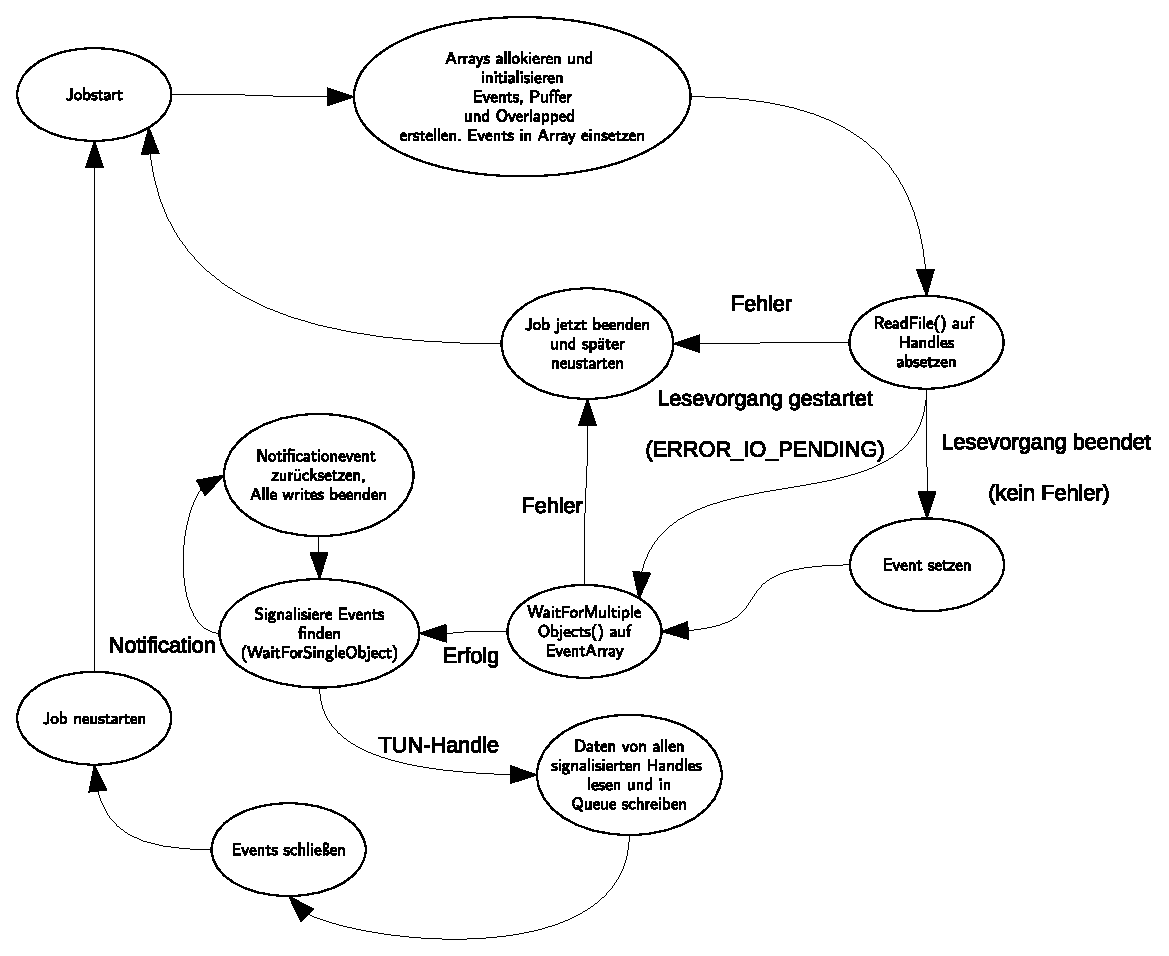
\includegraphics[width=\textwidth]{WaitForMultipleObjects.eps}
\caption{Zustände in handle\_plain() mittels WaitForMultipleObjects(), Variante 1}
\label{fig:WaitForMultipleObjects}
\end{figure}

\begin{figure}
\centering
\def\svgwidth{\columnwidth}
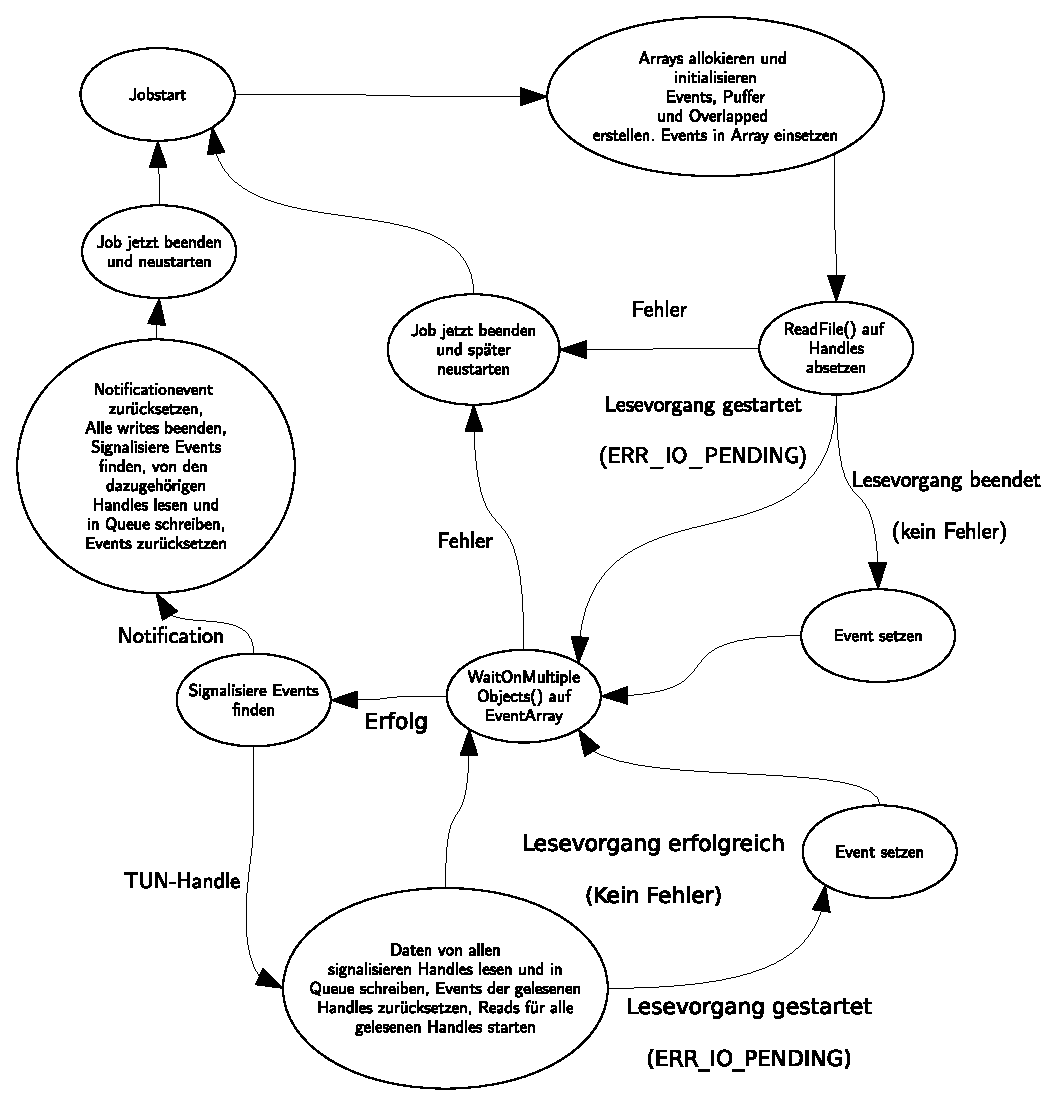
\includegraphics[width=\textwidth]{WaitForMultipleObjects2.eps}
\caption{Zustände in handle\_plain() mittels WaitForMultipleObjects(), Variante 2}
\label{fig:WaitForMultipleObjects2}
\end{figure}

\paragraph{Routing}
libipsec setzt für die von ihr installierten Routen standardmäßig das ''Gateway''
oder ''Next Hop''Feld nicht. Der Grund dafür ist, dass libipsec bisher nur auf
Betriebssytemen genutzt wurde, die echte Layer-3-Geräte implementieren und
daher keine Kollisionsdomäne über das Gerät erreichbar ist. Daher ergibt es keinen
Sinn das ''next hop''-Feld zu setzen.
Auf Windows ist dies jedoch, wie zuvor erläutert, nicht der Fall, da der TAP-Windows-Treiber
TUN-Geräte als Ethernet-Gerät emuliert.
Der Struct \texttt{route} is vom Typ \texttt{route\_entry\_t} und wird in der Funktion
\texttt{install\_route} genutzt, um die zu installierende Route zu bestimmen.
Das Gateway-Feld wird genutzt, um das Next-Hop-Feld der Routen im Routing-Table
zu setzen. 
Der TAP-Windows6-Treiber nutzt für IPv6 einen statische IP addresse im link-local-Bereich
der IPv6-Spezifikation.
Für IPv4 lässt sich die IP-Adresse des Adapters implizit konfigurieren, wie zuvor erklärt.
Das Object, welches mittels \texttt{host\_create\_from\_string} erstellt wird,
wird von der Funktion auf dem Heap abgelegt. Damit ist es auch nach dem Verlassen
des Funktionsblocks noch valide. Es wird automatisch beim Zerstören des
\texttt{route}-Objekts freigegeben.

\begin{lstlisting}[caption=Patch für die Routen-Installation von libipsec]
#ifdef __linux__
#elif defined(WIN32)
        /* Set out special gateway */
        family = route->src_ip->get_family(route->src_ip);
        switch(family)
        {
            case AF_INET:
            {
                /* For IPv4, the nxt hop is 169.254.128.128 (Configured next hop) */
                host_t *gw = host_create_from_string("169.254.128.128", 0);
                route->gateway = gw;
                break;
            }
            case AF_INET6:
            {
                /* For IPv6, the next hop is fe80::8 (TAP-Windows6 magic router gw) */
                host_t *gw = host_create_from_string("fe80::8", 0);
                route->gateway = gw;
                break;
            }
            default:
                DBG2(DBG_ESP, "Unknown Protocol family %d encountered. Not setting a next hop.", family);
                break;
        }
#else
        /* on Linux we cant't install a gateway */
        route->gateway = charon->kernel->get_nexthop(charon->kernel, dst, -1, src);
#endif
\end{lstlisting}

Das Plugin ''kernel-iph'' installiert Routen mit einer Metrik von 10.
Andere Software von Windows, die Routen installiert, benutzen eine höhere Metrik.

Routen mit einer Prefixlänge von 0 werden auf zwei Routen mit der Prefixlänge 1 aufgeteilt.
Dies wird gemacht um die Standardroute, welche ebenfalls eine Metrik von 10 besitzt,
nicht zu überschreiben.

Die Implementierung von handle\_plain() auf Windows unterstütz, wie die Implementierung
auf Linux und UNIX das Multiplexen von IO von mehreren TUN-Adaptern. Der Grund dafür ist,
dass verschiedene TUN-Implementierungen gegebenenfalls verschiedene Adapter für mehrere Tunnel
benötigen. Mit dem TAP-Windows-Treiber ist dies zwar nicht der Fall, es wurde der Vollständigkeit
halber jedoch mitemplementiert.

% libipsec router
% handle_plain
% notification event
% job
% handle_plain
% handle_esp
% up
% destroy
%kernel_libipsec_ipsec route installation
\subsubsection{libstrongswan}
Hier galt es das Öffnen, Konfigurieren und Schließen von TUN-Geräten
mit dem TAP-Windows-Treiber zu implementieren.

% Bezugsquelle für den Treiber
Der Treiber ist kompiliert auf der OpenVPN-Seite
verfügbar\footnote{\url{https://openvpn.net/index.php/open-source/downloads.html}}
und der Quellcode auf Github\footnote{\url{https://github.com/OpenVPN}}.
Die Basis für die Implementierung war hier der existierende Programmcode in
OpenVPN, spezifisch in  der Datei ''src/openvpn/tun.c.''.

\paragraph{TAP-Geräte erstellen}
Das Erstellen von TAP-Geräten ist im Moment nicht unterstützt. Der Grund dafür ist,
dass die Funktionalität von \texttt{devcon.exe} dafür nachgebaut werden müsste.
Des weiteren ist der Quellcode von \texttt{devcon.exe} zwar verfügbar\footnote{\url{https://github.com/Microsoft/Windows-driver-samples/tree/master/setup/devcon}},
aber nur unter einer proprietären Lizenz von Microsoft, der MS-PL\footnote{\url{https://github.com/Microsoft/Windows-driver-samples/blob/master/LICENSE}},
verfügbar. Eine Reimplementierung müsste Code aus dem Quellcode von \texttt{devcon.exe} nutzen,
welcher dann auch unter der MS-PL stünde. Die Verbreitung des Codes wäre dann nicht möglich,
da die MS-PL mit der GPL inkompatibel ist\footcite[][]{_gnu.org_2016}.
Da der Code unter der MIT-Lizenz beim strongSwan-Projekt eingereicht werden muss
und dann dual-lizensiert wird.
Wenn nur der Zugriff auf die benötigte API benutzt werden würde, so wäre es möglich,
die Unterstützung zu implementieren. Aus Zeitgründen wurde das nicht getan.

\paragraph{TAP-Geräte suchen}
Um das TAP-Gerät zu nutzen versucht der Code zuerst nach Netzwerkgeräten mit der ID ''tap0901'' zu suchen,
welche die ID für TAP-Geräte ist. Dies wird über die Registry getan. Hierbei wird
im Pfad \begin{lstlisting}[numbers=none]
HKEY_LOCAL_MACHINE\\SYSTEM\\CurrentControlSet\\Control\\Class\\{4D36E972-E325-11CE-BFC1-08002BE10318\}
\end{lstlisting}
nach Verbindungen gesucht, deren ''ComponentId''-Feld den Wert ''tap0901'' besitzen.
Bei passenden Schlüsseln wird der Wert ''NetCfgInstanceId'' an eine linked list
angehängt. Die NetCfgInstanceId identifiziert jeden Netzwerkadapter unter Windows
mittels einer einzigartigen ID.
Vor dem Beenden der Funktion wird die linked list zurückgegeben.
Diese Funktionalität ist in der Funktion get\_tap\_reg() in der Datei
''src/libstrongswan/networking/tun\_device.c'' gekapselt.

Der Code hierfür ist im Appendix unter \autoref{lst:get_tap_req} aufzufinden.

\paragraph{TAP-Geräte öffnen}
TAP-Geräte sind im Usermode über den Globalen Addressraum für Userspaceadapter
unter ''\textbackslash{}\textbackslash{}.\textbackslash{}\textbackslash{}Global\textbackslash{}\textbackslash{}\$NetCfgInstanceId.tap'' erreichbar.
\texttt{\$NetCfgInstanceId} steht hierbei für die vorher mit \texttt{get\_tap\_req()} gefundenen
\texttt{NetCfgInstanceId}-Werte der gefundenen TAP-Adapter.

\begin{lstlisting}[numbers=none]
CreateFile(device_path, GENERIC_READ \| GENERIC_WRITE, 0,
                    0, OPEN_EXISTING, FILE_ATTRIBUTE_SYSTEM | FILE_FLAG_OVERLAPPED, 0);
\end{lstlisting}

Das Handle kann nun genutzt werden um Pakete vom TAP-Gerät zu lesen und zu schreiben.
Mittels DeviceIoControl kann die Konfiguration des Geräts geändert werden,
wie die IP des virtuellen Routers, den Status des Geräts sowie der Modus des Geräts.

Für die Portierung wurden die \acp{FD} für Handles ausgetauscht und für das Benachrichtigen
über Änderungen in der Liste der TUN-Geräte wurde ein Event verwendet.

Für das Lesen und Schreiben vom und auf dem Handle wird ein Event benötigt,
welches in die OVERLAPPED-Struktur eingefügt wird. Das Event wird dynamisch mittels CreateEvent()
erstellt und nach der Nutzung mittels CloseHandle() geschlossen.

\paragraph{Ändern der MTU eines TAP-Geräts}
Der Treiber ermöglicht es,
die \ac{MTU} über die Windows-Registry zu ändern. Dort wird der Schlüssel ''MTU''
dafür genutzt. Er steht standardmäßig auf ''1500'', welches die Standard-\ac{MTU}
von Ethernet ist. Alternativ ist es vermutlich möglich, die Funktionen 
\texttt{SetIpInterfaceEntry}\footcite[][]{_setipinterfaceentry_2016} dafür zu nutzen, welche Teil der IP-Helper-\ac{API} ist.

\paragraph{Konfiguration eines TAP-Geräts}
Die Konfiguration eines TAP-Geräts geschieht mit den IOCTL-Werten aus ~/autoref{fig:tap-ioctls}.

Im Funktionskopf von \texttt{init\_tun} wird das Argument \texttt{name\_tmpl} übergeben,
welches auf Linux/UNIX den Anfang des Gerätenamens angibt, welcher dort \texttt{ipsec}
ist. Da das Erstellen von TAP-Geräten auf Windows in charon (noch) nicht implementiert
ist, wird es ignoriert.

Um ein TAP-Gerät erfolgreich zu konfigurieren muss zuerst eines gefunden werden. Das wird mit der Funktion
\texttt{find\_tap\_devices} getan. Sie sucht in der Registry, wie im Paragraph ''TAP-Geräte suchen''
beschrieben.
Nachdem alle TAP-Geräte gefunden wurden, wird versucht im globalen Geräteverzeichnis ein Handle
auf dem Gerät zu öffnen. Der Pfad zum Gerät wird hierbei aus dem globalen Geräteverzeichnis, der GUID des Geräts,
sowie der Endung ''.tap'' zusammengebaut.
Danach werden die folgenden Konfigurationsschritte ausgeführt.
\begin{itemize}
\item Das Gerät wird in den TUN-Modus setzen. Dabei werden als Parameter
die lokale IP (169.254.128.127), die IP des virtuellen Routers (169.254.128.128)
und die Netzmaske des entfernten Netzwerks (255.255.255.255) gesetzt. 
\texttt{(TAP\_WIN\_IOCTL\_CONFIG\_TUN)}
\item Die Überprüfung des ''Sender protocol address''-Feldes muss deaktiviert werden.\\
\texttt{(TAP\_WIN\_IOCTL\_CONFIG\_SET\_SRC\_CHECK)}
\item Der Adapter muss in den ''up''-Zustand gesetzt werden (einschalten). 
Nach dem Setzen des Zustands muss kurz gewartet werden um sicher zu gehen, dass das Gerät auch aktiv ist.\\
\texttt{(TAP\_WIN\_IOCTL\_SET\_MEDIA\_STATUS)}
\end{itemize}


\begin{lstlisting}[caption=Konfiguration eines TAP-Geräts,label=lst:tap-device-configuration]
/**
 * Initialize the tun device
 */
static bool init_tun(private_tun_device_t *this, const char *name_tmpl)
        [...]
#elif defined(WIN32)
        enumerator_t *enumerator;
        char *guid;
        BOOL success = FALSE;
        /* Get all existing TAP devices */
        linked_list_t *possible_devices = find_tap_devices();
        memset(this->if_name, 0, sizeof(this->if_name));

        /* Iterate over list */
        enumerator = possible_devices->create_enumerator(possible_devices);
        /* Try to open that device */
        while(enumerator->enumerate(enumerator, &guid))
        {
            if (!success){
                /* Set mode */
                char device_path[256];
                /* Translate dev name to guid */
                /* TODO: Fix. device_guid should be */
                snprintf (device_path, sizeof(device_path), "%s%s%s", USERMODEDEVICEDIR, guid, TAP_WIN_SUFFIX);

                this->tunhandle = CreateFile(device_path, GENERIC_READ | GENERIC_WRITE, 0,
                    0, OPEN_EXISTING, FILE_ATTRIBUTE_SYSTEM | FILE_FLAG_OVERLAPPED, 0);
                if (this->tunhandle == INVALID_HANDLE_VALUE)
                {
                    DBG1(DBG_LIB, "could not create TUN device %s", device_path);
                }
                else
                {
                    memcpy(this->if_name, guid, strlen(guid));
                    success = TRUE;
                }
            }
            else
            {
                break;
            }
            /* device has been examined or used, free it */
            free(guid);
        }

        /* possible_devices has been freed while going over the enumerator.
         * Therefore it is not necessary to free the elements in the list now.
         */
        enumerator->destroy(enumerator);
        possible_devices->destroy(possible_devices);
        /* If we didn't find one or could open one, we need to bail out.
         * We currently can not create new devices.
         */
        if (!success)
        {
            return FALSE;
        }
        /* set correct mode */
        /* We set a fake gateway of 169.254.254.128 that we route packets over
         The TAP driver strips the Ethernet header and trailer of the Ethernet frames
         before sending them back to the application that listens on the handle */
        struct in_addr ep[3];
        ULONG status = TRUE;
        DWORD len;
        /* Local address (just fake one): 169.254.128.127 */
        ep[0].S_un.S_un_b.s_b1 = 169;
        ep[0].S_un.S_un_b.s_b2 = 254;
        ep[0].S_un.S_un_b.s_b3 = 128;
        ep[0].S_un.S_un_b.s_b4 = 127;
        /*
         * Remote network. The tap driver validates it by masking it with the remote_netmask
         * and then comparing hte result against the remote network (this value here).
         * If it does not match, an error is logged and initialization fails.
         * (local & remote_netmask ? local)
         * The driver does proxy arp for this network and the local address.
         */
        /* We need to integrate support for IPv6, too. */
        /* Just fake a link local address for now (169.254.128.128) */
        ep[1].S_un.S_un_b.s_b1 = 169;
        ep[1].S_un.S_un_b.s_b2 = 254;
        ep[1].S_un.S_un_b.s_b3 = 128;
        ep[1].S_un.S_un_b.s_b4 = 128;
        /* Remote netmask (255.255.255.255) */
        ep[2].S_un.S_un_b.s_b1 = 255;
        ep[2].S_un.S_un_b.s_b2 = 255;
        ep[2].S_un.S_un_b.s_b3 = 255;
        ep[2].S_un.S_un_b.s_b4 = 255;

        if(!DeviceIoControl (this->tunhandle, TAP_WIN_IOCTL_CONFIG_TUN,
            ep, sizeof (ep),
            ep, sizeof (ep), &len, NULL))
        {
            DBG1 (DBG_LIB, "WARNING: The TAP-Windows driver rejected a TAP_WIN_IOCTL_CONFIG_TUN DeviceIoControl call.");
        }

        ULONG disable_src_check = FALSE;
        if(!DeviceIoControl(this->tunhandle, TAP_WIN_IOCTL_CONFIG_SET_SRC_CHECK,
                    &disable_src_check, sizeof(disable_src_check),
                    &disable_src_check, sizeof(disable_src_check), &len, NULL))
        {
            DBG1 (DBG_LIB, "WARNING: The TAP-Windows driver rejected a TAP_WIN_IOCTL_CONFIG_SET_SRC_CHECK DeviceIoControl call.");
        }
        ULONG driverVersion[3] = {0 , 0, 0};
        if(!DeviceIoControl(this->tunhandle, TAP_WIN_IOCTL_GET_VERSION,
                    &driverVersion, sizeof(driverVersion),
                    &driverVersion, sizeof(driverVersion), &len, NULL))
        {
            DBG1(DBG_LIB, "WARNING: The TAP-Windows driver rejected a TAP_WIN_IOCTL_GET_VERSION DeviceIoControl call.");
        }
        else
        {
            DBG1(DBG_LIB, "TAP-Windows driver version %d.%d available.", driverVersion[0], driverVersion[1]);
        }
        /* Set device to up */

        if (!DeviceIoControl (this->tunhandle, TAP_WIN_IOCTL_SET_MEDIA_STATUS,
                &status, sizeof (status),
                            &status, sizeof (status), &len, NULL))
        {
            DBG1 (DBG_LIB, "WARNING: The TAP-Windows driver rejected a TAP_WIN_IOCTL_SET_MEDIA_STATUS DeviceIoControl call.");
        }

            /* Give the adapter 2 seconds to come up */

        sleep(2);
        return TRUE;
        [...]
}
\end{lstlisting}


\paragraph{Lesen und Schreiben vom Adapter}
Beim Öffnen des Adapters wurde ein Handle erstellt.
Durch asynchrone Lese- und Schreiboperationen mittels ReadFile() und WriteFile()
unter Benutzung von \texttt{OVERLAPPED}-Strukturen und Events lassen sich Pakete
lesen und schreiben.

\paragraph{tun\_device\_t}
Die Klasse für TUN-Geräte musste für Windows angepasst werden.
Spezifisch mussten neue Funktionen zum Lesen und Schreiben implementiert werden,
sowie Attribute geändert werden.
Auf Windows wird ein Objekt vom Typ \texttt{HANDLE} genutzt, statt eines \ac{FD}.

\begin{lstlisting}[caption=Code für das Erstellen von tun\_device\_t,label=lst:tun_device_t_create]
tun_device_t *tun_device_create(const char *name_tmpl)
{
	private_tun_device_t *this;

	INIT(this,
		.public = {
			.read_packet = _read_packet,
			.write_packet = _write_packet,
			.get_mtu = _get_mtu,
			.set_mtu = _set_mtu,
			.get_name = _get_name,
                        /* For WIN32, that's a handle. */
#ifdef WIN32
                        .get_handle = _get_handle,
#else
			.get_fd = _get_fd,
#endif /* WIN32 */
			.set_address = _set_address,
			.get_address = _get_address,
			.up = _up,
			.destroy = _destroy,
		},
#ifdef WIN32
                .tunhandle = NULL,
#else

		.tunfd = -1,
		.sock = -1,
#endif /* WIN32 */
	);

	if (!init_tun(this, name_tmpl))
	{
		free(this);
		return NULL;
	}
#ifdef WIN32
	DBG1(DBG_LIB, "opened TUN device: %s", this->if_name);
#else
	DBG1(DBG_LIB, "created TUN device: %s", this->if_name);

	this->sock = socket(AF_INET, SOCK_DGRAM, 0);
	if (this->sock < 0)
	{
		DBG1(DBG_LIB, "failed to open socket to configure TUN device");
		destroy(this);
		return NULL;
	}
#endif /* WIN32 */
	return &this->public;
}
\end{lstlisting}


\begin{lstlisting}[caption=Relevanter code für tun\_device\_t->destroy(),label=lst:tun_device_t_destroy]
METHOD(tun_device_t, destroy, void,
	private_tun_device_t *this)
{
#ifdef WIN32
        /* close file handle, destroy interface */
        CloseHandle(this->tunhandle);
#else
        [...]
#ifdef __FreeBSD__
        [...]
#endif
        [...]
#endif
	DESTROY_IF(this->address);
	free(this);
}
\end{lstlisting}
Beim Destruktur für die Klasse musste nur statt dem Zerstören eines TUN-Geräts
nur das Handle des TAP-Geräts geschlossen werden.
% callbacks
% synchronous
% WaitForMultipleObjects
% komplexe Änderungen des Verhaltens von kernel-libipsec

\subsubsection{kernel-iph}
kernel-iph ist ein Plugin für \texttt{charon}, das das Kernel-Interface
für die Verwaltung von IP-Adressen und Routen implementiert.

Ursprünglich war das Verwalten von IP-Adressen im Master-Zweig nicht implementiert.
Eine vollständige Implementierung existiert im Zweig \texttt{win-vip}, die in den Zweig 'windows-libipsec'
gemerged wurde, um eine vollständige Implementierung dort zu erhalten.

Nachgerüstet werden musste Code zum Beachten des \texttt{charon.install\_virtual\_ip\_on} Parameters
der in der Datei \texttt{strongswan.conf} definiert werden kann und den libipsec nutzt um
die Installation der empfangenen IP-Adresse(n) auf den richtigen Adapter zu erzwingen.
Der Code kopiert den Adapternamen während der Initialisierung des Plugins, daher
ändert ein Ändern des Parameters während der Laufzeit nicht die Schnittstelle,
auf die die IP-Adresse installiert werden würde.

Die bekannten IP-Adressen werden in kernel-iph in einer Datenstruktur gespeichert,
um sie schnell nachschlagen zu können und Berechnungen zu tätigen. Die Struktur
wird einerseits durch manuelles Einfügen und Entfernen von selbstinstallierten Adressen
bewerkstelligt, als auch durch Events, die die Anwendung über ein Handle
vom Kernel empfängt.

\begin{lstlisting}[caption=Ergänzung zu private\_kernel\_iph\_net\_t,label=lst:kernel_iph]
/**
 * Private data of kernel_iph_net implementation.
 */
struct private_kernel_iph_net_t {
        [...]
        /**
         * Whether to install virtual IPs
         */
        bool install_virtual_ip;

        /**
         * Where to install virtual IPs
         */

        char *install_virtual_ip_on;
};
\end{lstlisting}

Die Klasse für das Plugin \texttt{kernel-iph} wurde um zwei Attribute für die Installation
von \ac{IP}-Adressen erweitert. Einerseits ein bool'scher Wert, der die Installation
aktiviert und deaktiviert und andererseits einen \texttt{char *}, der genutzt wird
um das Gerät zu konfigurieren, auf welchem alle \ac{IP}-Adressen installiert werden sollen.

\begin{lstlisting}[caption=Code für add\_ip,label=lst:kernel_iph_add_ip]
METHOD(kernel_net_t, add_ip, status_t,
    private_kernel_iph_net_t *this, host_t *vip, int prefix, char *name)
{
        if (!this->install_virtual_ip)
        {    /* disabled by config */
            return SUCCESS;
        }
        MIB_UNICASTIPADDRESS_ROW row;
        u_long status;
        iface_t *iface = NULL, *entry = NULL;

        /* Print out all known interfaces */
        enumerator_t *enumerator = this->ifaces->create_enumerator(this->ifaces);
        while(enumerator->enumerate(enumerator, &entry))
        {
            DBG1(DBG_KNL, "interface %s\n index: %d\n description %s\n type %d", entry->ifname, entry->ifindex, entry->ifdesc, entry->iftype);
        }
        enumerator->destroy(enumerator);
        /* name of the MS Loopback adapter */
        if (!this->install_virtual_ip_on || this->ifaces->find_first(this->ifaces, (void*)iface_by_name,
                        (void**)&iface, this->install_virtual_ip_on) != SUCCESS)
        {
            name = "{DB2C49B1-7C90-4253-9E61-8C6A881194ED}";
        }
        else
        {
            name = this->install_virtual_ip_on;
        }
        host2unicast(vip, prefix, &row);

        row.InterfaceIndex = add_addr(this, name, vip, TRUE);
        if (!row.InterfaceIndex)
        {
            DBG1(DBG_KNL, "interface '%s' not found", name);
            return NOT_FOUND;
        }

        status = CreateUnicastIpAddressEntry(&row);
        if (status != NO_ERROR)
        {
            DBG1(DBG_KNL, "creating IPH address entry failed: %lu", status);
            remove_addr(this, vip);
            return FAILED;
        }
        return SUCCESS;
}
\end{lstlisting}

Die Methode \texttt{add\_ip} in~\autoref{lst:kernel_iph_add_ip} des \texttt{kernel-iph}-Plugins musste angepasst werden.
Ursprünglich war sie nur ein Stub, der \texttt{return NOT\_SUPPORTED;} enthielt.
Nach dem der Quellcode aus dem Zweig \texttt{win-vip} gemerged wurde, wurde der Code erweitert
um die Attribute \texttt{install\_virtual\_ip\_on} und \texttt{install\_virtual\_ip} zu beachten.
Dabei wird zuerst überprüft, ob \ac{IP}-Adressen überhaupt installiert werden
sollen und danach, ob eine Schnittstelle konfiguriert ist.
Wenn eine Schnittstelle konfiguriert ist, dann wird sie in der internen
Schnittstellenliste von \texttt{kernel-iph} mittels \texttt{this->ifaces->find\_first()}
nachgeschlagen um zu überprüfen ob sie existiert. Wenn sie existiert,
wird die \ac{IP}-Adresse mittels \texttt{host2unicast} und
\texttt{CreateUnicastAddressEntry} darauf installiert. Wenn sie nicht existiert, 
wird die \ac{IP}-Adresse auf dem Loopback-Adapter installiert.

\begin{lstlisting}[caption=Code für del\_ip,label=lst:kernel_iph_del_ip]
METHOD(kernel_net_t, del_ip, status_t,
    private_kernel_iph_net_t *this, host_t *vip, int prefix, bool wait)
{
        if (!this->install_virtual_ip)
        {    /* disabled by config */
            return SUCCESS;
        }

        MIB_UNICASTIPADDRESS_ROW row;
        u_long status;

        host2unicast(vip, prefix, &row);

        row.InterfaceIndex = remove_addr(this, vip);
        if (!row.InterfaceIndex)
        {
            DBG1(DBG_KNL, "virtual IP %H not found", vip);
            return NOT_FOUND;
        }

        status = DeleteUnicastIpAddressEntry(&row);
        if (status != NO_ERROR)
        {
            DBG1(DBG_KNL, "deleting IPH address entry failed: %lu", status);
            return FAILED;
        }

        return SUCCESS;
}
\end{lstlisting}

\begin{lstlisting}[caption=Ergänzung zu kernel\_iph\_net\_create(),label=lst:kernel_iph_create]
*
 * Described in header.
 */
kernel_iph_net_t *kernel_iph_net_create()
{
        [...}
        .install_virtual_ip = lib->settings->get_bool(lib->settings,
                        "%s.install_virtual_ip", TRUE, lib->ns),
        .install_virtual_ip_on = lib->settings->get_str(lib->settings,
                        "%s.install_virtual_ip_on", NULL, lib->ns),
       [...]
}
\end{lstlisting}

Für das Implementieren des Codes für den TAP-Treiber werden Magic Numbers benötigt,
welche sich im Quellcode von OpenVPN finden lassen. Diese wurden übernommen
und in einer Header-Datei angelegt.
Teilweise wurden auch die Konstanten für die Erzeugung der Namen der Events für
das IO-Multiplexen dort abgelegt. Die Datei ist im Appendix unter \autoref{lst:libstrongswan-win32.h}
zu finden.

Der gesamte gepatchte Quellcode von strongSwan ist auf der CD unter strongSwan/ zu finden
Der Patch ansich ist unter patches/strongSwan/tap-handling.patch zu finden.

\subsection{TAP-Treiber}
% openvpn
% kompatibilität
% Treiber-patches upstream
Im Zuge der \ac{BA} wurde ein Patch für den TAP-Windows-Treiber entwicklelt, um die
Prüfung der Quell-IP der ARP-Requests zu deaktivieren. Das ist erforderlich, um mit der
virtuellen IP des Clients mit dem entfernten IP-Netzwerk kommunizieren zu können.


\subsubsection{Bauen und Installieren des Treibers}
Um den Treiber zu bauen, wird zuallererst der Quellcode benötigt, sowie die
Vorraussetzungen, welche auf der Github-Seite dort aufgelistet sind.
Die aktuellen Minimalvorraussetzungen sind Python 2.7, das Microsoft Windows 7 WDK (Windows Driver Kit)
und ein Windows Code signing certificate.
Das Zertifikat muss nicht valid sein, wenn der Treiber nicht produktiv ausgerollt
werden soll. Der Grund ist, dass unter Windows das Überprüfen der Treibersignatur deaktiviert
werden kann, aber der Treiber muss trotzdem signiert sein. Der Trust-path muss aber nicht
zu einem öffentlichen Trust Anchor (eine CA) führen. Um den Treiber signieren zu können,
wird die gesamte Trust Chain benötigt, sowie der private Schlüssel des Zertifikats.
Um ein Zertifikat mit dem dazugehörigen privaten Schlüssel importieren zu können,
müssen die Dateien in einen PKCS\#12-Container gepackt werden. Dieser kann mit 
OpenSSL erstellt werden, zum Beispiel mit diesem Befehl:
\begin{lstlisting}[caption=OpenSSL PKCS\#12]
openssl pkcs12 -export -in key key.key -in certificate.pem -out pkcs12.p12
\end{lstlisting}
Die mit diesem Befehl erstellte Datei pkcs12.p12 kann dann durch einen Doppelklick auf sie
in den Windows importiert werden.
Folgend ist ein beispielhafter Befehl zum Bau des Treibers.
\begin{lstlisting}[caption=TAP-Windows bauen]
python buildtap.py -c -b -d --cert="csc" --sign --crosscert="C:\Users\Noel\certs\rootca.pem"
\end{lstlisting}
Die Ausgabe des Befehls listet die Kompilierung, sowie das Signieren der Dateien auf.
% Hier noch Ausgabe der Kompilierung aufführen, sowie welche Teile kritisch sind.
Wie zu sehen ist, muss das Root-CA-Zertifikat als Datei vorhanden sein.
Das Code Signing certificate wird nur mit seinem Common Name angegeben.
Damit das WDK es findet, muss es in ''Eigene Zertifikate'' zu finden sein.
\begin{figure}
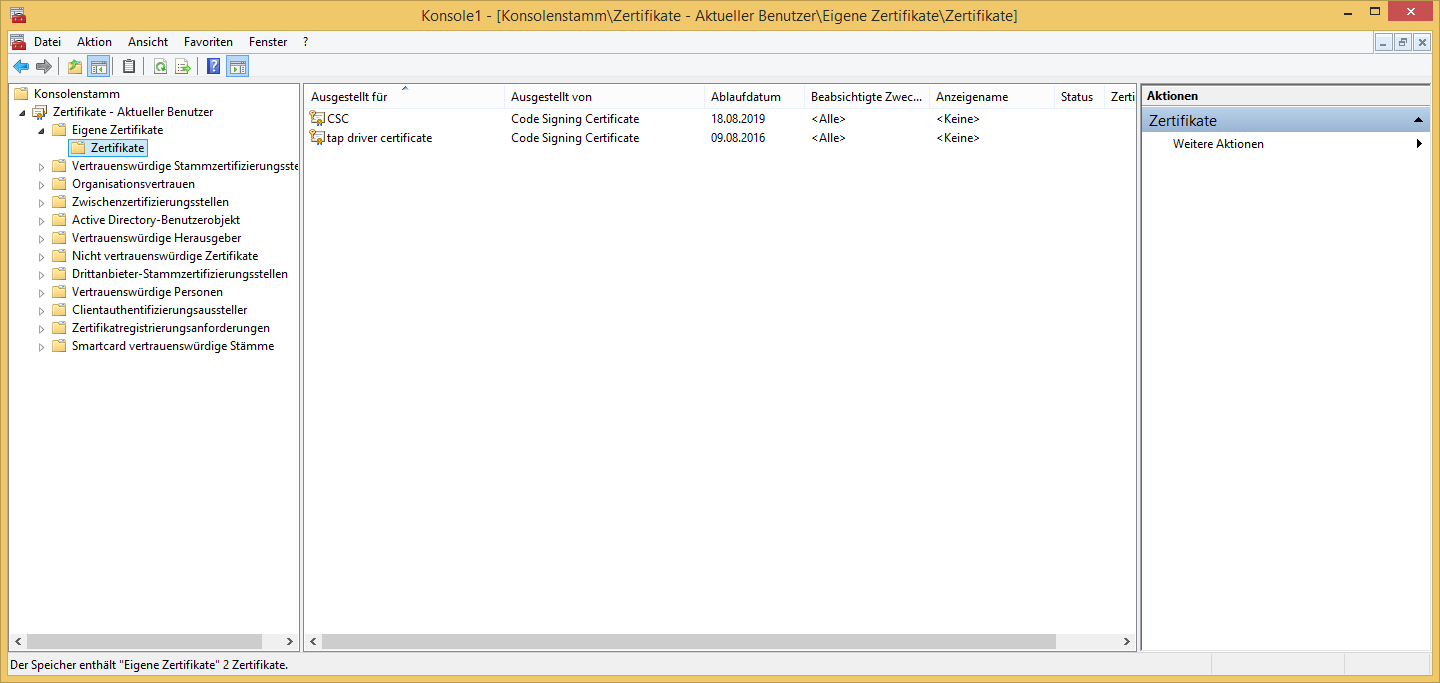
\includegraphics[scale=0.33]{/home/thermi/FH-Stuff/UNITS-8/Bachelorarbeit/Bachelorarbeit/Bilder/Eigene_Zertifikate.png}
\caption{Eigene-Zertifikate-Menü}
\label{fig:Eigene-Zertifikate-Menue}
\end{figure}

Mit Windows im Testmodus kann der Treiber geladen werden und TAP-Geräte konnen
mittels tapinstall.exe (Was eigentlich \texttt{devcon.exe} ist). Die Datei ist im Quellcode des
Treibers nicht mitenthalten. Sie kann jedoch durch die Installation des Treiber-Pakets
von der OpenVPN-Webseite erhalten werden. Nach der Installation des Pakets
ist die Datei unter \textit{C:\textbackslash{}Program Files\textbackslash{}TAP-Windows\textbackslash{}bin\textbackslash{}tapinstall.exe}
zu finden und kann zur Erstellung und zum Löschen von TAP-Geräten genutzt werden.

Der erste Parameter ist ''install'' oder ''remove''. Der Pfad zur .inf-Datei
über den Treiber muss beim Erstellen eines Geräts angegeben werden. Hier im Beispiel
ist es die Datei, die mittels des Python-Skripts erstellt wurde. Bei der Installation
dieses Treibers wird der kompilierte Treiber installiert, welcher sich unter 
\texttt{C:\textbackslash{}Users\textbackslash{}Noel\textbackslash{}tap-driver\textbackslash{}dist\textbackslash{}amd64\textbackslash{}OemVista.inf}
befindet.

\begin{lstlisting}[caption=Erstellung eines TAP-Geraets]
"C:\Program Files\TAP-Windows\bin\tapinstall.exe" install "C:\Users\Noel\tap-driver\dist\amd64\OemVista.inf" tap0901
\end{lstlisting}

\begin{lstlisting}[caption=Löschung aller TAP-Geraete]
"C:\Program Files\TAP-Windows\bin\tapinstall.exe" remove tap0901
\end{lstlisting}

\paragraph{ABI}
Die \ac{ABI} des Treibers ist undokumentiert. Im Folgenden ist eine Auflistung
der Funktionen der \ac{ABI}. Sie wurden aus der Datei ''src/device.c'' extrahiert
und aufgeschlüsselt. Für mehr Informationen bezüglich des Verhaltens und der
genauen Eingabeparameter sollte die Datei konsultiert werden.

\begin{table}
\tiny
\begin{tabularx}{\textwidth}{|c|c|c|c|X|X|}\firsthline
IOCtl & Makro & Eingabe & Ausgabe & Zweck & Kommentar \\ \hline
1 & TAP\_WIN\_IOCTL\_GET\_MAC & NULL & char[6] & Gibt die MAC-Adresse des Geräts zurück & \\ \hline
2 & TAP\_WIN\_IOCTL\_GET\_VERSION & NULL & ULONG[3] & Gibt die Version des Treibers zurück & \\ \hline
3 & TAP\_WIN\_IOCTL\_GET\_MTU & NULL & ULONG & Gibt die \ac{MTU} des Geräts zurück & \\ \hline
4 & TAP\_WIN\_IOCTL\_GET\_INFO & NULL & N/A & Gibt Informationen über den Adapter zurück
& Ist laut Code für NDIS6 nicht implementiert \\ \hline 
5 & TAP\_WIN\_IOCTL\_CONFIG\_POINT\_TO\_POINT & IPADDR[2] (2*4 CHAR) & NULL & Setzt das Gerät in den Point-To-Point-Modus
& \\ \hline
6 & TAP\_WIN\_IOCTL\_SET\_MEDIA\_STATUS & ULONG & NULL & Setzt das Gerät in den ''Up'' oder ''Down''-Zustand & \\ \hline
7 & TAP\_WIN\_IOCTL\_CONFIG\_DHCP\_MASQ & IPADDR[4] (4*4 CHAR) & NULL & Aktiviert den internen DHCP-Server, DHCP-IP-Adresse, DHCP-Netzmaske, DHCP-Server-IP, Leasetime & \\ \hline
8 & TAP\_WIN\_IOCTL\_GET\_LOG\_LINE & allokierter String (char *) & NULL & Gibt eine Debug-Log-Zeile zurück & \\ \hline
9 & TAP\_WIN\_IOCTL\_CONFIG\_DHCP\_SET\_OPT & char[256] & NULL & Setzt die DHCP-Optionen & \\ \hline
10 & TAP\_WIN\_IOCTL\_CONFIG\_TUN & IPADDR[3] (3*4 char) & NULL & Setzt das Gerät in den TUN-Modus, lokale IP, entferntes Netzwerk, entfernte Netzmaske & \\ \hline
11 & TAP\_WIN\_IOCTL\_CONFIG\_SET\_SRC\_CHECK & ULONG & NULL & Deaktiviert oder Aktiviert den ARP-Source-Check. ''0'' deaktiviert ihn. ''1'' aktiviert ihn (Standard) & \\ \hline
\end{tabularx}
\caption{TAP-Windows-Treiber IOCtls}
\label{fig:tap-ioctls}
\end{table}

\paragraph{Patch}
Bei der Entwicklung des Patchs wurde viel Zeit darauf verwendet die funktionalen
Komponenten zu finden, die bei der Verarbeitung von \ac{ARP}-Requests ausgeführt werden,
sowie die Codepfade zu finden, die bei der Verarbeitung von Daten abgelaufen werden.

Der entwickelte Patch deaktiviert die Überprüfung der Quell-IP der \ac{ARP}-Requests, die
vom Treiber verarbeitet werden. Wenn die Überprüfung erfolgreich war, so wird der ARP-Request
beantwortet und dem Kernel wird damit mitgeteilt, wie die MAC-Adresse des virtuellen Routers lautet.

Für die Implementierung der Routen wurde die Nutzung eines virtuellen Routers gewählt,
da das Routen aller \ac{IP}-Adressen über das Gerät die \ac{ARP}-Tabelle des Clients
mehr gefüllt hätte und eine \ac{ARP}-Adressabfrage bei jeder Kommunikation mit einer neuen
\ac{IP}-Adresse zu Folge hätte.

Der Patch wurde entwickelt, indem nach der Behandlung von \ac{ARP}-Paketen im
Quellcode des Treibers gesucht wurde. Dafür wurde nach ''ARP'' und ''arp'' mittels
''grep'' im Quelltext gesucht. Dabei wurde die Funktion ''ProcessARP'' in ''src/txpath.c''
gefunden, in der \ac{ARP}-Requests verarbeitet werden. In dieser Funktion
werden verschiedene Felder des Pakets überprüft, unter anderem das ''Sender protocol address''-Feld.

Die Überprüfung des ''Sender protocol address''-Felds wurde optional gemacht, 
wobei es standardmäßig aktiviert ist. Die Kontrolle dieses
Feldes kann über ein IOCTL-Wert gesteuert werden. Der momentane Zustand der Option
wird im Adapter-Kontext des TAP-Adapters gespeichert.

Er wurde 2016-08-15 in der OpenVPN Community auf freenode im Kanale \#openvpn-meeting besprochen
und bekam ein feature-ack. Ein Code-ack steht noch aus. Das Ticket ist unter
\url{https://community.openvpn.net/openvpn/ticket/721} zu finden.

Der komplette Patch ist auf der CD unter 
''patches/tap-windows/0001-implement-source-ip-check.patch'' zu finden.


\subsection{Test des Codes}
Zum Testen des Codes wurde er mit der implementierten TAP-Treiber-Unterstützung
kompiliert und im Netzwerk getestet, sowie mit TravisCI in einer standardisierten
Umgebung gebaut. Dabei werden verschiedene Standardkonfiguriatonen auf Linux und auf Mac OSX
kompiliert, sowie von Linux auf Windows crosscompiled und überprüft, ob es
Fehler während des Build-Vorgangs auftragen. TravisCI überprüft alle Builds
auf Fehler und sendet eine Benachrichtigung aus, wenn der Build-Vorgang fehlgeschlagen ist.

Im Testszenario für den Netzwerktest wurde der Quellcode auf Linux für Windows 64-Bit cross kompiliert
und in einer \ac{VM} mit Windows 8.1 ausgeführt.

Die gebauten Binärdateien wurden über ein geteiltes Verzeichnis der \ac{VM}
zugänglich gemacht. Danach wurden sie in ''C:\textbackslash{}\textbackslash{}Users\textbackslash{}\textbackslash{}Thermi\textbackslash{}\textbackslash{}bin
kopiert und in 'cmd' mit Administratorrechten ausgeführt. 
Die nötige Dateistruktur sollte wie in Abbildung \ref{fig:Ordnerstruktur} 
auf Seite \pageref{fig:Ordnerstruktur} aussehen.

Im Unterordner ''swanctl'' befindet sich die Dateien ''swanctl.conf'',
sowie die Ordner ''bliss'', ''ecdsa'', ''pkcs8'', ''pkcs12'', ''pubkey'', ''rsa'', ''x509'',
''x509aa'', ''x509ac'', ''x509ca'', ''x509crl'' und''x509ocsp''.
Im Ordner ''rsa'' befindet sich der private Schlüssel für den Client. Im Ordner
''x509'' befindet sich das Zertifikat des Clients und im Ordner ''x509ca'' alle
\ac{CA}-Zertifikate vom Zertifikat des Clients bis zum selbstsignierten Wurzelzertifikat,
sowie das Zertifikat der Server-\ac{CA}.

\begin{figure}
\def\svgwidth{\columnwidth}
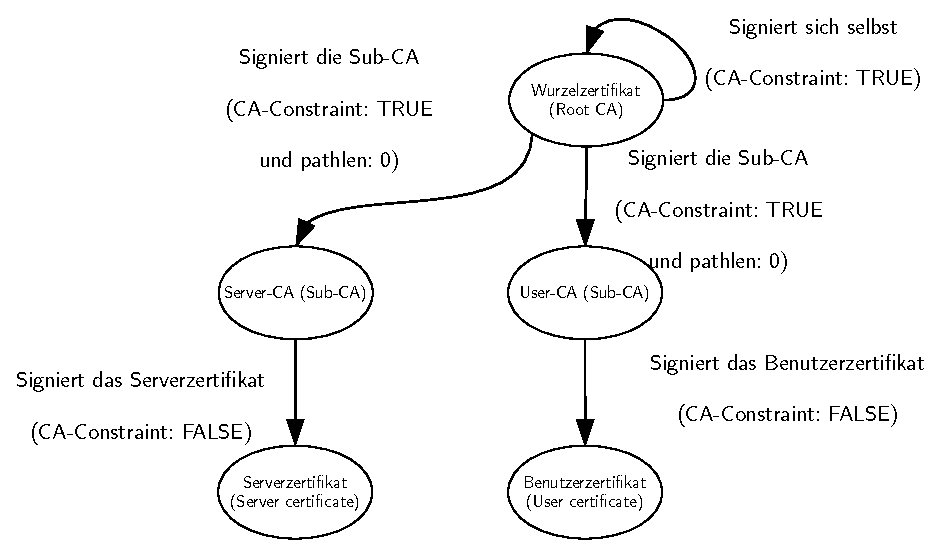
\includegraphics[width=\textwidth]{CA-Struktur.eps}
\caption{Eine exemplarische CA-Struktur}
\label{fig:CA-Struktur}
\end{figure}

Die Datei \texttt{this\_log} wurde von der Logger-Konfiguration des Dienstes erstellt.
Hierbei wurde zuerst \texttt{charon-svc.exe}
in einem ersten Fenster ausgeführt. In einem zweiten Fenster wurde die Konfiguration geladen
und der Tunnelaufbau mittels \texttt{swanctl.exe} gestartet. Hierbei wurden \texttt{swanctl.exe --load-all} und \texttt{swanctl --i --child bar}.
Nach dem Testen wurde der Tunnel, sollte \texttt{charon-svc.exe} nicht gecrasht sein, mit \texttt{swanctl -t --ike foo}
beendet, sodass keine virtuellen IP-Adressen oder Routen für den nächsten Test zurückbleiben.

Wenn \texttt{charon-svc.exe} getötet wird, während ein Tunnel mit Routen und \ac{IP}-Adressen
aufgebaut ist, so verbleiben IP-Adressen und Routen auf dem Adapter, was verhindern kann dass
dieselben Routen und \ac{IP}-Adressen wieder installiert werden. Das führt dazu, dass der
Aufbau der CHILD\_SA fehlschlägt und ein neuer Tunnel nicht aufgebaut werden kann.
In diesem Fall müssen sie manuell über die Nutzung von \texttt{route delete}} oder \texttt{netsh}
gelöscht werden oder Windows neu gestartet werden.

OpenSSL auf Windows wird für die Kryptographie benötigt und liegt nicht in den Standardsuchpfaden
für Bibliotheken und Header. Aus diesem Grund werden die Header und Bibliotheken
über LDFLAGs in Include-Pfade auf der Kommandozeile übergeben.

Die Bibliotheken von OpenSSL wurden durch die Installation von OpenVPN beschafft.
Bei der Installation von OpenVPN werden direkt die Bibliotheken von OpenSSL mitinstalliert.

\begin{centering}
\begin{figure}
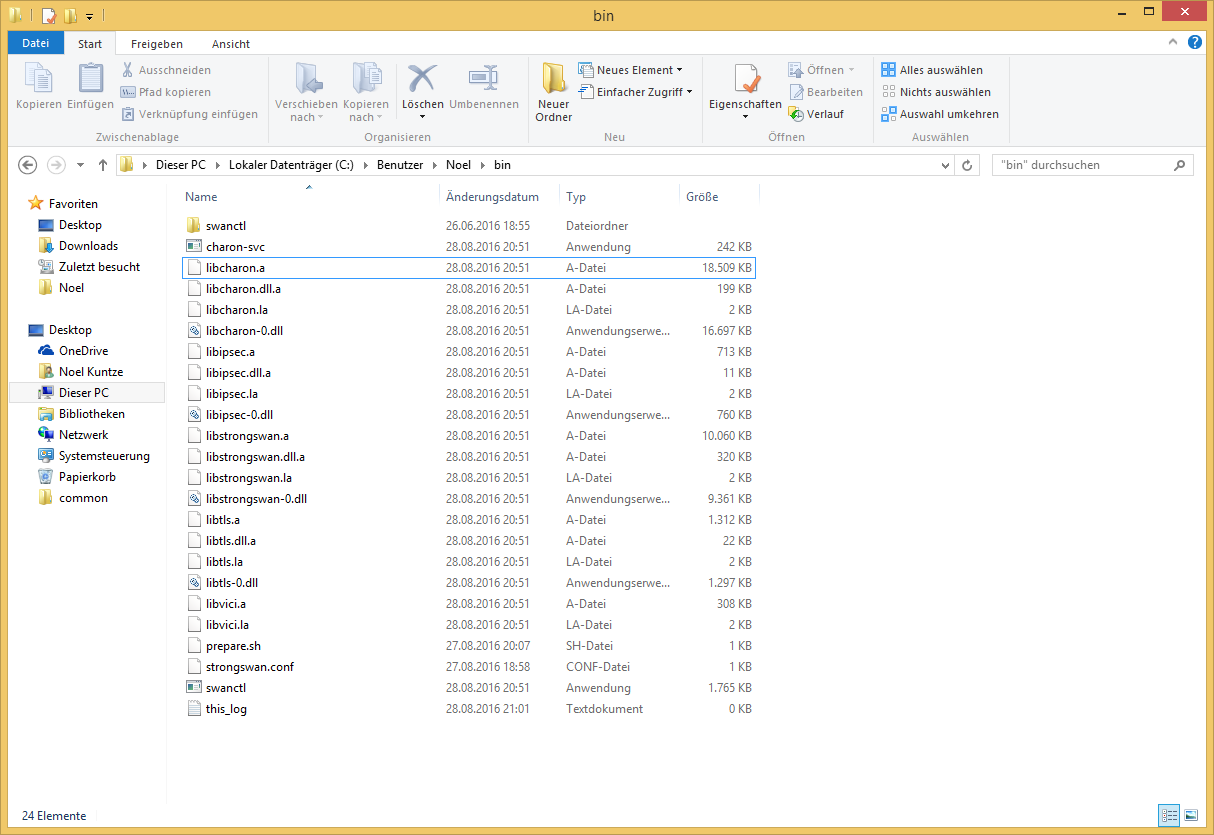
\includegraphics[width=\textwidth]{Bilder/Ordnerstruktur.png}
\caption{Ordnerstruktur nach dem Kopieren der Dateien}
\label{fig:Ordnerstruktur}
\end{figure}
\end{centering}

\begin{centering}
\begin{figure}
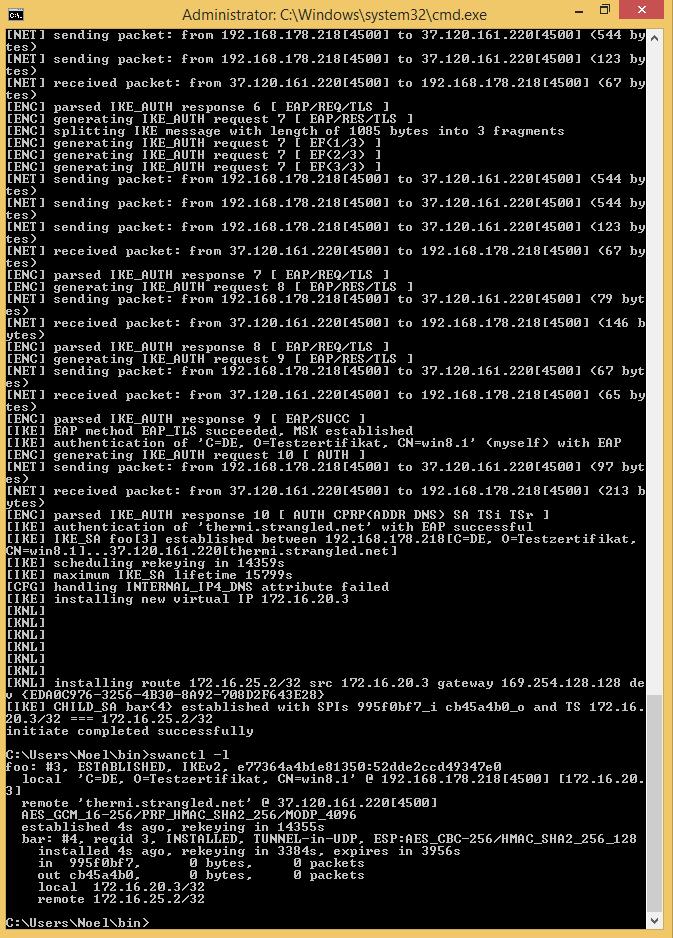
\includegraphics[width=\textwidth]{Bilder/Aufbau_und_swanctl_-l.png}
\caption{Ausgabe des Tunnelaufbaus und swanctl -l}
\label{fig:swanctl-l}
\end{figure}
\end{centering}

Die unter \autoref{lst:strongswan.conf} und \autoref{lst:swanctl.conf} bereitgestellten
Konfigurationen wurden zur Konfiguration des Dienstes genutzt.

\pagebreak

\begin{lstlisting}[caption=./configure und make]
./configure --host=x86_64-w64-mingw32 --prefix=/ --libdir=/bin --bindir=/bin --sbindir=/bin --disable-defaults --enable-monolithic --enable-static --enable-svc --enable-ikev2 
--enable-ikev1 --enable-nonce --enable-pem --enable-pkcs1 --enable-x509 --enable-openssl --enable-socket-win --enable-kernel-wfp --enable-kernel-iph --enable-pubkey --enable-swanctl 
--with-swanctldir=swanctl --with-strongswan-conf=strongswan.conf --enable-libipsec --enable-kernel-libipsec --enable-eap-tls --enable-mschapv2 --enable-eap-peap --enable-eap-gtc 
--enable-eap-dynamic --enable-eap-identity --enable-md4 --enable-ipseckey --enable-dnscert --enable-files --enable-sha3 host_alias=x86_64-w64-mingw32 CC=x86_64-w64-mingw32-gcc 
CFLAGS=-g -O2 -Wall -Werror -Wno-pointer-sign -Wno-format-security -Wno-format -mno-ms-bitfields -I/home/thermi/FH-Stuff/UNITS-8/Bachelorarbeit/win32-headers/files/include/ 
LDFLAGS=-L/home/thermi/FH-Stuff/UNITS-8/Bachelorarbeit/win32-headers/files/lib/ -L/home/thermi/FH-Stuff/UNITS-8/Bachelorarbeit/win32-headers/files/bin/
make clean && make
\end{lstlisting}

Der Befehl konfiguriert den strongSwan Quellcode zum Bauen der benötigten Plugins, sowie einiger
Extras für die Authentifizierung und dazu den 64-Bit Compiler des MINGW32-Projekts zu nutzen.

Der Code wurde getestet, indem versucht wurde eine VPN-Verbindung zu einem \ac{IKE}-Peer
unter meiner Kontrolle aufzubauen. Der ausgehandelte \ac{TS} wurde so gewählt, dass
die Beschränkung von Route based VPNs keine Rolle spielen.
Die genutzte Konfiguration ist im Appendix unter \autoref{lst:swanctl.conf}
und \autoref{lst:strongswan.conf} zu finden.

\subsection{Test der Verbindung}
Das Testen der Verbindung wurde durch durch einfaches Pingen über die Verbindung bewerkstelligt.
Dabei wird durch Dumpen der Pakete mit tcpdump und Wireshark überprüft, ob die
\ac{ARP}-Requests auf dem TUN-Adapter beantwortet werden und ob das Paket auf dem
anderen Endpunkt auftaucht. Des weiteren werden die Traffic-Counter der \acp{SA} überprüft,
um zu überprüfen, ob die Pakete jemals verarbeitet wurden.

\subsection{Leistung}

Die Leistung der Implementierung wurde mittels einer Verbindung vom Gast zum Host der Testplattform ermittelt.
Als Testumgebung wurde eine Virtualbox-\ac{VM} genutzt, die auf einem Computer
mit einem Intel(R) Core(TM) i7-3820 CPU ausgerüstet ist. Diese \ac{CPU} hat vier Kerne.
Die verschiedenen Prozesse wurden nicht auf bestimmte Kerne gepinnt. Der \ac{CPU}-Governor
wurde in den Performance-Modus gestellt. Die Messpunkte
wurden mittels einer simplen Software in \texttt{Python 2.7.12} ermittelt, die im Abstand
von einer Sekunde die CPU-Auslastung der Kerne ermittelt. Für die Konfiguration des
Initiators und des Responders wurden die Konfigurationen aus~\autoref{lst:speedtest-initiator-config}
und~\autoref{lst:speedtest-responder-config} genutzt.
Die Ciphersuite \texttt{null-sha1} wurde gewählt, um den Overhead bei der Verarbeitung
der Pakete in \texttt{charon} zu minimieren.

\begin{lstlisting}[label=lst:speedtest-initiator-config,caption=Initiator-Konfiguration für den Geschwindigkeitstest]
connections {
        speedtest {
                version = 2
                fragmentation = yes
                remote_addrs = 192.168.178.43
                mobike = yes
                proposals = aes256gcm16-prfsha256-modp4096
                vips = 0.0.0.0
                local {
                        auth = psk
                        id = speedtest-initiator
                }
                remote {
                        auth = psk
                        id = speedtest-responder
                }
                children {
                        speedtest-child {
                                esp_proposals = null-sha1
                                remote_ts = 172.17.0.1
                        }
                }

        }
}

secrets {
        ike-speedtest {
                secret = speedtest
                id = speedtest-responder
                id = speedtest-initiator
        }
}
\end{lstlisting}
\begin{lstlisting}[label=lst:speedtest-responder-config,caption=Responder-Konfiguration für den Geschwindigkeitstest]
connections {
        speedtest {
                version = 2
                fragmentation = yes
                mobike = yes
                proposals = aes256gcm16-prfsha256-modp4096
                pools = alpha
                local {
                        auth = psk
                        id = speedtest-responder
                }
                remote {
                        auth = psk
                        id = speedtest-initiator
                }
                children {
                        speedtest-child {
                                esp_proposals = null-sha1
                                local_ts = 172.17.0.1
                        }
                }
                
        }
}

pools {
        alpha {
                addrs = 172.16.16.1-172.16.16.10
        }
}
secrets {
        ike-speedtest {
                secret = speedtest
                id = speedtest-initiator
                id = speedtest-responder
        }
}
\end{lstlisting}

Die CHILD\_SA wird vom Initiator mithilfe von \texttt{swanctl} aufgebaut. Das Kommando
ist in~\autoref{lst:swanctl-speedtest} sichtbar.
\begin{lstlisting}[label=lst:swanctl-speedtest,caption=Kommando für den Tunnelaufbau des Geschwindigkeitstests]
swanctl -i --child speedtest-child
\end{lstlisting}

\begin{lstlisting}[label=lst:speedtest-host-iperf-server,caption=Kommando für den Start des iperf-Servers]
iperf3 -f m -s 
\end{lstlisting}

\begin{lstlisting}[label=lst:speedtest-guest-iperf-client,caption=Kommando für den Start des iperf-Clients]
iperf3 -t 60 -c 172.17.0.1
\end{lstlisting}
Der \texttt{iperf3}-Server wurde mit dem Kommando aus~\autoref{lst:speedtest-host-iperf-server}
gestartet und der Client mit dem Kommando aus~\autoref{lst:speedtest-guest-iperf-client}.


Damit das Routing auf dem Initiator korrekt funktioniert, wurde ihm mittels eines pools
und \texttt{Config Mode} eine ''virtuelle'' \ac{IP}-Adresse zugewiesen. Dies war und ist
nötig, damit die \acp{SP} auf dem Initiator installiert werden können.
Die IP \texttt{172.17.0.1} ist eine lokale IP auf dem resolver. Sie wurde als
einer der Teilnehmer beim Geschwindigkeitstest genutzt. 
Als Software wurde \texttt{iperf3} in Version \texttt{3.1.3} genutzt.
Die Binärdatei für den Windows-Gast wurde von \url{https://iperf.fr/iperf-download.php} bezogen.
Auf dem Linux-Host wurde \texttt{iperf3} in Version \texttt{3.1.3} von einem Archlinux-Mirrorserver mittels
\texttt{pacman} bezogen.

Der \texttt{iperf3}-Server wurde auf dem Host in einer Bash-Shell mittels
dem Befehl in~\autoref{lst:speedtest-host-iperf-server} gestartet.
\begin{figure}[h!]
\caption{Statistik über iperf3-Leistung durch den Tunnel}
\begin{tikzpicture}
\pgfplotstableread{benchmark_guest.txt}\benchmarkguest
\pgfplotstableread{iperf_server_normalized.txt}\benchmarkthroughput
\begin{axis}[
title=CPU-Last und Durchsatz bezogen auf Zeit,
xlabel={Zeit in Sekunden seit Start der Messung},
ylabel={CPU-Last in Prozent},
legend pos=south east,
width=\textwidth,
height=\textwidth,
legend entries={Gast-CPU 0, Gast-CPU-2, Gast-CPU-3}
]

\addplot table[x=time,y=cpu0] {\benchmarkguest};
\addplot table[x=time,y=cpu1] {\benchmarkguest};
\addplot table[x=time,y=cpu2] {\benchmarkguest};
\end{axis}
\begin{axis}[
hide x axis,
axis y line*=right,
ylabel={Durchsatz in MegaBit pro Sekunde},
legend entries={Durchsatz von iperf3},
legend pos=south west,
width=\textwidth,
height=\textwidth
]
\addplot [draw=green] table[x=time,y=throughput] {\benchmarkthroughput};
\end{axis}
\end{tikzpicture}
\label{fig:iperf-statistics}
\end{figure}

In~\autoref{fig:iperf-statistics} wurde der Durchsatz einer \texttt{iperf3}-Messung
durch den konfigurierten Tunnel dargestellt.

Die Leistung des TAP-Adapters scheint auf etwa 60 MegaBit pro Sekunde beschränkt zu sein.
Dies ist hier jedoch nicht einer möglichen schlechte Implementierung der IO-Operationen in charon
geschuldet, sondern dem TAP-Windows6-Treiber selbst. Es ist seit langem bekannt, dass die
Leistung des Treibers sehr schlecht ist\footcite[][]{_openvpn_2015}.
Es fällt auf, dass die \ac{CPU}-Last nie auf 100\%, sondern nur auf 90\%
steigt und die erste CPU des Gasts in der Mitte des Tests eine relativ geringe Auslastung von
70\% bis 40\% erfährt.

\subsection{Notwendige Features für Nutzung als RW auf Windows}

\paragraph{DNS-Resolver}
Um DNS-Server installieren zu können, muss die Unterstützung dafür noch implementiert werden.
DNS-Einträge werden in IKE mittels \texttt{Config Mode} oder \ac{CP} an den Initiator übertragen
und dort konfiguriert.
\paragraph{Windows 10}
Windows verwaltet die DNS-Resolvereinträge für jede Schnittstelle einzeln, statt
global in einer Datei. Seit Windows 10 wird jeder konfigurierte Resolver nach einem Namen
gefragt und die schnellste Antwort wird genutzt. Das ist gefährlich, da in VPNs 
zu Unternehmensnetzen für gewöhnlich private DNS-Zonen für die Adressierung
von Computern im Unternehmensnetzwerken genutzt werden. Ein Angreifer kann
den Verkehr zwischen dem Host und dem DNS-Resolver in einem unprivilegierten
Netzwerk abhören und so in Erfahrung bringen mit welchen internen Hosts kommuniziert wird.
Des weiteren kann er diese Anfragen beantworten und die Race-Condition zwischen den
Resolvern versuchen zu gewinnen, um den Verkehr zum Rechner umzuleiten und
den Host so anzugreifen. Dies kann unter Windows mittels Firewallregeln
verhindert werden, die mittels \ac{WFP} verwaltet werden.

\paragraph{Authentifizierung für VICI}
In die \ac{VICI}-\ac{API} von charon ist keine Authentifizierung integriert.
Auf Windows wird die \ac{VICI}-\ac{API} über einen TCP-Socket genutzt, der auf Port 4502
horcht. charon bindet den Dienst dabei an die \ac{IP}-Adresse \texttt{127.0.0.1}.
Damit ist der Dienst für alle lokalen Anwendungen erreichbar und jedes Programm
kann charon konfigurieren und kontrollieren.
Um dem vorzubeugen müsste eine Authentifizierungsschicht in \ac{VICI} implementiert werden.
Unter Linux/UNIX macht charon die \ac{VICI}-\ac{API} nur über einen Unix-Socket
zugänglich, welcher mittels den konfigurierten Zugriffsrechten standardmäßig
nur für den ''root''-Benutzer zugänglich ist. Die Anwendungen, die als ''root''-Benutzer
ausgeführt werden, sind in der Regel ausgewählt und vertrauenswürdig.  Wenn eine Anwendung
als ''root''-Benutzer ausgeführt wird, hat sie in der Regel, wenn keine weiteren Sicherheitsmaßnahmen getroffen
wurden, bereits Zugriff auf alle Systemfunktionen und kann beliebige Aktionen im System ausführen.
Der Wiki-Artikel über \ac{VICI} zeigt die Unsicherheit des \ac{VICI}-Protokolls auf.
\begin{quote}
The VICI protocol runs over a reliable transport protocol. As the protocol itself currently does not provide any security or authentication properties, it is recommended to run it over a UNIX socket with appropriate permissions.
\end{quote}\cite[][]{_vici_2016}
\paragraph{Dynamische Authentifizierungsaufforderungen}
Charon beherrscht noch keine Weitergabe von Authentifizierungsaufforderungen,
die über XAUTH oder EAP empfangen werden und nach mehreren Strings fragen.
Ein solches Szenario ist die Authentifizierung mittels einer PIN und eines Passworts.
charon kann im Moment nur einen einzelnen String über XAUTH oder EAP übertragen.
Ein weiteres Problem ist, dass eine PIN, die zum Konfigurationszeitpunkt
eingegeben wird, nicht zwingend zum Authentifizierungszeitpunkt gültig ist.

\subsection{Probleme}
Während der \ac{BA} wurden mehrere Probleme identifiziert, die mit unbekanntem
Verhalten von Funktionen und Standards zusammenhängen.
\paragraph{C-Standard}
Eines dieser Probleme ist, dass der C-Standard die Deklaration einer Variable
direkt nach einem ''case'' eines switch-cases nur erlaubt, wenn die Deklaration
in einem Codeblock stattfindet.
Der folgende Code produziert eine Fehlermeldung:
\begin{lstlisting}[caption=Problematik mit C-Standard,label=c-standard]
void main() {
    int foo = 0;
    
    switch(foo)
    {
        case 0:
            char *bar;
            break;
        default:
            break;
    }

}
\end{lstlisting}
Die Problematik kann umgangen werden, wenn der Code im case mit geschweiften Klammern
umfasst wird, wie hier:
\begin{lstlisting}[caption=Abhilfe für Problematik mit C-Standard,label=c-standard-fix]
void main() {
    int foo = 0;
    
    switch(foo)
    {
        case 0:
        {
            char *bar;
            break;
        }
        default:
            break;
    }
}
\end{lstlisting}
\begin{filecontents*}{c-standard-error.tex}
test.c: In Funktion »main«:
test.c:7:13: Fehler: eine Marke kann nur Teil einer Anweisung sein, und eine Deklaration ist keine Anweisung
             char *bar;
             ^~~~
\end{filecontents*}

\lstinputlisting[caption=Fehlermeldung von gcc,label=c-standard-error,inputencoding=utf8/latin1]{c-standard-error.tex}

Interessanterweise ist eine Deklaration in einem ''case'' erlaubt, jedoch nur
nicht direkt nach der Deklaration des ''case''.
Daher funktioniert dieser Code auch.

\begin{lstlisting}[caption=Abhilfe mittels NOOP,label=c-standard-noop]
void main() {
    int foo = 0;
    
    switch(foo)
    {
        case 0:
            ;
            char *bar;
            break;
        default:
            break;
    }
}

\end{lstlisting}
\paragraph{WaitForSingleObject()}
Wie erläutert wird WaitForMultipleObjects() genutzt, um die IO-Operationen
zu multiplexen. Diese Funktion beendet im Programmcode mit dem Wert ''1'',
was bedeuted dass das zweite Objekt (In C werden Arrays von 0 auf indexiert.)
im Array signalisiert wurde. Bei der Überprüfung mit WaitForSingleObject() ist das jedoch nicht
der Fall. Wenn das Event signalisiert wäre, dann würde der folgende Aufruf
den Wert ''WAIT\_OBJECT\_0'' (0x0) zurückgeben:
\begin{lstlisting}
WaitForSingleObject(event_array[offset], 0)
\end{lstlisting}]
Das ist jedoch nicht der Fall. Der Aufruf beendet mit ''WAIT\_TIMEOUT'' (0x102, 258),
was bedeuted, dass das Event nicht signalisiert ist. Wenn der Rückgabewert
ignoriert wird, dann befindet sich im Puffer kein valides IPv4-Packet.

Das Problem ist besonders evident bei der Betrachtung des Debug-Logs,
welches sich auf Seite \pageref{lst:debug-log} finden lässt.
Es wird vom Code in auf Seite \pageref{lst:handle-plain-windows} ausgegeben.

\paragraph{GetLastError()}
Des weiteren gibt die Funktion ''GetLastError()'' den Fehlerwert 0 zurück, wenn sie nicht
direkt nach dem Funktionsaufruf, der den Fehlerstatus setzte, aufgerufen wird.
Es ist irrelevant, ob zwischen dem Aufruf von ''GetLastError()'' nur eine einfache Zuweisung
oder eine If-Abfrage steht.
Dies ergibt keinen Sinn, da sich der Fehlerstatus scheinbar ändert, ohne dass
eine Funktion aufgerufen wird, die das tun könnte.
